\chapter{BACKGROUND}
\label{chp:background}
In its simplest form sparse matrix vector multiplication is the operation $y=Ax$, where A is an $M \times N$, $x$ is a vector of length $N$, and $y$ is a vector of length $M$. As Equation 2.1 shows, matrix vector multiplication is a series of dot products.
\begin{equation}
\left[\begin{IEEEeqnarraybox*}[][c]{,c,}
{y_1}\\
{y_2}\\
{y_3}\\
{y_4}\\
{y_5}\\
{y_6}\\
{y_7}\\
{y_8}
\end{IEEEeqnarraybox*}\right]
=
\left[\begin{IEEEeqnarraybox*}[][c]{,c,}
{A_{11}x_1}{+A_{14}x_4}{+A_{17}x_7}\\
{A_{25}x_5}{+A_{28}x_8}\\
{A_{32}x_3}{+A_{33}x_3}{+A_{36}x_6}{+A_{37}x_7}\\
{A_{41}x_1+A_{45}x_5}\\
{A_{53}x_3+A_{54}x_4+A_{57}x_7+A_{58}x_8}\\
{A_{62}x_2+A_{65}x_5}\\
{A_{72}x_2+A_{73}x_3+A_{76}x_6+A_{78}x_8}\\
{A_{83}x_3+A_{84}x_4+A_{85}x_5+A_{86}x_6}
\end{IEEEeqnarraybox*}\right]
=
\left[\begin{IEEEeqnarraybox*}[][c]{,c/c/c/c/c/c/c/c,}
{A_{11}} & 0 & 0 & {A_{14}} & 0 & 0 & {A_{17}} & 0\\
0 & 0 & 0 & 0 & {A_{25}} & 0 & 0 & {A_{28}} \\
0 & {A_{32}} & {A_{33}} & 0 & 0 & {A_{36}} & {A_{37}} & 0 \\
{A_{41}} & 0 & 0 & 0 & {A_{45}} & 0 & 0 & 0\\
0 & 0 & {A_{53}} & {A_{54}} & 0 & 0 & {A_{57}} & {A_{58}}\\
0 & {A_{62}} & 0 & 0 & {A_{65}} & 0 & 0 & 0\\
0 & {A_{72}} & {A_{73}} & 0 & 0 & {A_{76}} & 0 & {A_{78}}\\
0 & 0 & {A_{83}} & {A_{84}} & {A_{85}} & {A_{86}} & 0 & 0
\end{IEEEeqnarraybox*}\right]
\left[\begin{IEEEeqnarraybox*}[][c]{,c,}
{x_1}\\
{x_2}\\
{x_3}\\
{x_4}\\
{x_5}\\
{x_6}\\
{x_7}\\
{x_8}
\end{IEEEeqnarraybox*}\right]
\label{eqn:example}
\end{equation}
\par Sparse matrices differ from dense matrices in that they contain mostly (usually more than 99\%) zeros. For example, consider the matrix representation of the Facebook friends graph [\cite{prelim:zuckerburg}]. Each row contains non-zero values representing friend connections and zero values representing non-friends, or people you do not know. Being friends with .1\% of Facebook users would require being friends with 1 million people, an impressive feat. In other words, from the time you started reading this paper 100 people have joined Facebook and are not friends with you. The average user has 300 friends. For this reason, sparsity of matrices is usually measured in elements per row rather than a percent. The percent sparsity of the matrix keeps growing but the number of non-zero elements per row stays roughly constant.
\section{Coordinate Format (COO)}
\par Dense matrices can be stored as an array of values. However, if sparse matrices were stored this way they would require orders of magnitude more space than a simple alternative. The alternative, coordinate format (COO), stores 3 arrays: a row index array, a column index array, and a value array. By convention, row and column indices are 4 byte (32-bit) integers. Values are either single-precision (32-bit) or double-precision (64-bit) floating point values. For simplicity, this paper only concerns itself with double precision values. Using the example matrix, the COO format would be:\\
ROW:    0, 0, 0, 1, 1, 2, 2, 2, 2, 3, 3, 4, 4, 4, 4, 5, 5, 6, 6, 6, 6, 7, 7, 7, 7 \\ 
COLUMN: 0, 3, 6, 4, 7, 1, 2, 5, 6, 0, 4, 2, 3, 6, 7, 1, 4, 1, 2, 5, 7, 2, 3, 4, 5\\ 
VALUE: $A_{11}$, $A_{14}$, $A_{17}$, $A_{25}$, $A_{28}$, $A_{32}$, $A_{33}$, $A_{36}$, $A_{37}$, $A_{41}$, $A_{45}$, $A_{53}$, $A_{54}$, $A_{57}$, $A_{58}$, $A_{62}$, $A_{65}$, $A_{72}$, $A_{73}$, $A_{76}$, $A_{78}$, $A_{83}$, $A_{84}$, $A_{85}$, $A_{86}$ \par
You will notice that the elements are traversed in row-major form. Row-major traversal starts at the left most element of the first row ($A_{11}$). Then proceeds to the next element on its right ($A_{14}$). After arriving at the last element of a row the next element would be the left most element in the row below it ($A_{25}$). This is simple and convenient, but not a required way to traverse the matrix. 
\par Calculating SpMV with this matrix format is straight forward and much faster than if the whole matrix was used. SpMV takes $nnz$ multiplications and $nnz-M$ additions, where $nnz$ is the number of non-zero values in the matrix and $M$ is the height of the matrix. This totals $2\times nnz - M$ floating point operations. However, the convention in the field uses a slightly incorrect but simpler $2\times nnz$ to report performance, which we use to report our performance. The difference is usually only a slight over estimate of the actual performance, but the difference could be significant if $nnz/M$ (number of non-zero elements per row) is small.
\begin{figure}
\centering
\begin{tikzpicture}[blueRect/.style={draw,rectangle,fill=blue!30,thick,minimum width=2cm, minimum height=.7cm}, %
redRect/.style={draw,trapezium,fill=red!30,thick,minimum width=3cm, minimum height=.7cm}, %
data/.style={draw,trapezium,fill=blue!30,thick,trapezium left angle=70,trapezium right angle=-70,minimum height=.7cm,minimum width=1cm}]
%\clip (-1.15cm,.45cm) rectangle (\linewidth, -6.35cm);
\tikzstyle{line} = [draw, thick, -latex' ,shorten >=2pt];
\node[draw,ellipse,fill=blue!30, inner ysep=0](A){\shortstack{$A$ Matrix \\ Data}};
\node[blueRect, inner ysep=0](B)[right=of A]{Decoder};
\node[data, inner ysep=0](C)[right=of B]{\shortstack{Column\\Data}};
\node[blueRect, inner ysep=0](D)[below=of C]{\shortstack{$x$ Memory\\Request}};
\node[data, inner ysep=0](E)[below=of D]{\shortstack{$x$ Vector \\Data}};
\node[data, inner ysep=2](F)[below=of A]{\shortstack{Matrix\\Value\\Data}};
\node[data, inner ysep=0, yshift = .2cm](G)[below=of B]{\shortstack{Row\\Data}};
\node[blueRect, inner ysep=0, yshift = .2cm](H)[below=of G]{Multiplier};
%\node[data](I)[below=of H]{Product};
\node[draw,diamond,fill=blue!30, inner sep=0, yshift=.5cm](J)[below=of H]{\shortstack{Intermediator;\\To Result\\Or Adder?}};
%\node[data](K)[below=of J]{
\node[blueRect, yshift = -1cm](L)[above left=of J]{Adder};
\node[draw,ellipse,fill=blue!30, inner ysep=0](M)[right=of J]{\shortstack{Result\\$y$ Vector}};
%\node(N)[left=of L]{};

\tikzstyle{every path}=[line]
\path    (A)  --  (B);
\path  (B) -- (C);
\path (C) -- (D);
\path (D) -- (E);
\path (B) -- (F);
\path (B) -- (G);
\path (F) |- (H);
\path (G) -- (H);
\path (E.west) |- (H);
\path (H) -- (J);
\path (J) -| (L);
\path (L) -| (J.north west);
\path (J) -- (M);

\end{tikzpicture}
\caption[SpMV dataflow diagram]{The dataflow is mostly the same for all SpMV implementations. Often the matrix is not stored in COO format and needs be decoded into each matrix's column, row and floating point value. As the dataflow shows, the processor needs the column data before accessing the $x$ vector data.}
\label{fig:dataflow}
\end{figure}%
\section{CPU}
Computing SpMV on any platform follows the dataflow outlined in \figurename~\ref{fig:dataflow}. It only takes a couple lines to write an SpMV function in c:
\begin{verbatim}
void spmv(double* y, double* x, int* row, int* column, double* value, int nnz,
        int height){
    // Zero the y vector.
    for(int i = 0; i < height; ++i){
        y[i] = 0;
    }
    // Compute SpMV.
    for(int i = 0; i < nnz; ++i){
        y[row[i]] = y[row[i]] + value[i] * x[column[i]];
    }
}
\end{verbatim}
In fact, this simple code is not that much worse than highly optimized CPU implementations.
\par The sparsity of the matrix causes CPUs to perform below their potential. A recent Intel publication using 2 Xeon E5-2699 v3 processors show an average performance of 1 TFLOP (1,000 GFLOPs) for matrix matrix multiplication but publishes an average performance of 27 GFLOPS for SpMV.
\par To understand this look at the equation~\ref{eqn:example} again and count the number of times each value is accessed. The values in the matrix only get accessed once and the values in the vector only get accessed a couple times. This remains the same for large matrices, because, as mentioned, the number of non-zero values per row ($nnz/M$) often grows slowly for larger matrices. This means the computation operations to memory operations ratio is low. Compare this to matrix-matrix multiplication where the ratio is high and each CPU can perform at 500 GFLOPs, almost the limit of the CPU.
\par The effect of this small ratio effects the CPU less when everything can fit in cache. Although it still exists, because L3 cache has some latency.
\par There exists several optimizations to improve the performance of SpMV. We cover CPU and GPU optimizations first. As we cover techniques we also look at how they could apply to FPGA implementations. If you are impatient feel free to skip ahead to Chapter~\ref{chp:method}, which talks about our approach to computing SpMV on FPGAs.

\section{Compressed Sparse Row Format (CSR)}
The first SpMV optimization, compressed sparse row (CSR), is the simplest. The optimization compresses the row indices. The column and value arrays are the same as COO. A compressed row array replaces the row array. The row array usually does not change from one element to the next and when it does it only changes by increasing the index by one. CSR format stores the traversal index of the first element of each row instead of the row index of each element. The traversal index equals the number of non-zero elements that are traversed before the current element is reached. We use the term traversal index to prevent confusion when mentioning row and column index. This change saves up to 4 bytes per element or 25\% over COO format. The CSR format of the matrix in equation~\ref{eqn:example} is shown: \\
COMPRESSED ROW: 3, 5, 9, 11, 15, 17, 21, 25 \\
COLUMN: 0, 3, 6, 4, 7, 1, 2, 5, 6, 0, 4, 2, 3, 6, 7, 1, 4, 1, 2, 5, 7, 2, 4, 5\\ 
VALUE: $A_{11}$, $A_{14}$, $A_{17}$, $A_{25}$, $A_{28}$, $A_{32}$, $A_{33}$, $A_{36}$, $A_{37}$, $A_{41}$, $A_{45}$, $A_{53}$, $A_{54}$, $A_{57}$, $A_{58}$, $A_{62}$, $A_{65}$, $A_{72}$, $A_{73}$, $A_{76}$, $A_{78}$, $A_{83}$, $A_{84}$, $A_{85}$, $A_{86}$ \par
\section{Block Sparse Row Format (BSR)}
\par Compression schemes often take advantage of the clumpy structures of sparse matrices. Blocking or register blocking stores dense sub-blocks of the matrix together. This again reduces the matrix storage size by storing fewer indices. Some explicit zeros are added to complete the sub-blocks.
\par The block sparse row (BSR) storage format is one such block storage scheme. It stores the row and column indices of the top left of the block and stores the values of the block in row major form. This matrix format is usually coupled with a second matrix; meaning the matrix is the sum of 2 matrices one in BSR format the other in CSR or COO. Formats that use the sum of two smaller matrices are called hybrid formats. We have pessimistic view of hybrid formats, because this results in performing SpMV on 2 matrices, both of which are sparser than the original. In general, the rest of the field agrees with this and tries to minimize this negative effect by minimizing the size of the second matrix. \par
The block sparse for the example in equation \ref{eqn:example} is shown:\\
ROW: 0, 0, 2, 2, 4, 4, 4, 6, 6, 6\\
COLUMN: 3, 6, 0, 4, 1, 3, 6, 1, 3, 5 \\
Value: \{$A_{14}$, $0$, $0$, $A_{25}$\}, \{$A_{17}$, $0$, $0$, $A_{28}$\}, \{$0$, $A_{32}$, $A_{41}$, $0$\}, \{$0$, $A_{36}$, $A_{45}$, $0$\}, \{$0$, $A_{53}$, $A_{62}$, $0$\}, \{$A_{54}$, $0$, $0$, $A_{65}$\}, \{$A_{57}$, $A_{58}$, $0$, $0$\}, \{$A_{72}$, $A_{73}$, $0$, $A_{83}$\}, \{$0$, $0$, $A_{84}$, $A_{85}$\}, \{$A_{76}$, $0$, $A_{86}$, $0$\}\\
Secondary COO Matrix:\\
ROW: 0, 2, 2, 6\\
COLUMN: 0, 2, 6, 7\\
VALUE: $A_{11}$, $A_{33}$, $A_{37}$, $A_{78}$\par
This simplified example does not actually save space because of the extra zeros stored, however, bitmaps can be used instead storing explicit zero values.
\section{Cache Blocking}
\par CPU optimizations also include changing the matrix traversal for better vector reuse. BSR does this to a small extent. One method called Cache blocking traverses large sub-blocks individually before proceeding to the next block. The dimensions of the block are around the size of available cache. This method has similarities to our row column row (RCR) traversal, introduced later in Chapter \ref{chp:compression}. The Cache Blocking in COO format for the example in equation \ref{eqn:example} is shown:\\
ROW: 0, 0, 2, 2, 3, 0, 1, 1, 2, 2, 3, 4, 4, 5, 6, 6, 7, 7, 4, 4, 5, 6, 6, 7, 7\\
COLUMN: 0, 3, 1, 2, 0, 6, 4, 7, 5, 6, 4, 2, 3, 1, 1, 2, 2, 3, 6, 7, 4, 5, 7, 4, 5\\
VALUE: $A_{11}$, $A_{14}$, $A_{32}$, $A_{33}$, $A_{41}$,
$A_{17}$, $A_{25}$, $A_{28}$, $A_{36}$, $A_{37}$, $A_{45}$,
$A_{53}$,  $A_{54}$, $A_{62}$, $A_{72}$, $A_{73}$, $A_{83}$, $A_{84}$,
$A_{57}$, $A_{58}$, $A_{65}$, $A_{76}$, $A_{78}$, $A_{85}$, $A_{86}$\par
\section{GPU}
%TODO: fit in average 14 GFLOPS performance
Before discussing storage formats specific to GPUs, it is important to understand GPUs play the computation game differently than CPUs. To show this let us compare a high end CPU (Intel Xeon E5-2699 v3) and a high-end GPU (Nvidia Tesla K40). The GPU has a max throughput of 1.66 TFLOPS (double precision). The CPU has a max throughput of 518 GFLOPS (double precision). The GPU has 1.5MB of cache. The CPU has 45MB of cache. The cache is growing every generation as well. The previous Tesla (Fermi) had 768KB of cache. The previous Xeon(E7-8890) had 38MB of cache. The GPU is a vector processor making it hard to get good performance on unstructured computation. The GPU supports up to 30720 threads whereas the CPU supports 36 threads. \par
    When using a COO format based GPU implementation each thread processes $nnz/30720$ values. Some synchronization occurs to ensure the correct $y$ values are stored. This implementation performs relatively well due to the good load balancing. However, this format does hardly any $x$ vector reuse. In fact, if you disable the cache, you get almost identical performance [\cite{prelim:bell}].\par
    In CSR format, the GPU assigns a thread or group of threads per row. This method achieves much better vector reuse and therefore better performance. One way to think about this is that all the threads start by processing values on the left side of the matrix and proceed to the right. This means different threads will process elements with the same column index at around the same time, leading to $x$ values being reused before getting flushed from the cache.

\section{ELLPACK}
\par To enable better performance \cite{prelim:bell} introduced ELLPACK, a storage format designed for vector processors. ELLPACK stores the same number of values for each row. Rows with fewer values than the row with the most values are padded with zeros.
\begin{equation}
    \textrm{\shortstack{Matrix\\Data}}
    =
    \left[\begin{IEEEeqnarraybox*}[][c]{,c/c/c/c,}
            A_{11} & A_{14} & A_{17} & 0 \\
            A_{25} & A_{28} & 0 & 0 \\
            A_{32} & A_{33} & A_{36} & A_{37} \\
            A_{41} & A_{45} & 0 & 0 \\
            A_{53} & A_{54} & A_{57} & A_{58} \\
            A_{62} & A_{65} & 0 & 0 \\
            A_{72} & A_{73} & A_{76} & A_{78} \\
            A_{83} & A_{84} & A_{85} & A_{86}
    \end{IEEEeqnarraybox*}\right]
    ,
    \textrm{\shortstack{Column\\Indices}}
    =
    \left[\begin{IEEEeqnarraybox*}[][c]{,c/c/c/c,}
            0 & 3 & 6 & \times \\
            4 & 7 & \times & \times \\
            1 & 2 & 5 & 6 \\
            0 & 4 & \times & \times \\
            2 & 3 & 6 & 7 \\
            1 & 4 & \times & \times \\
            1 & 2 & 5 & 7 \\
            2 & 3 & 4 & 5
    \end{IEEEeqnarraybox*}\right]
\end{equation} \par
Like CSR each thread computes one row of the matrix. However, the ELLPACK matrix is stored in column major order. This enables coalesing memory access. Coalesing memory access essentially means different threads are accessing the same cache lines. The ELLPACK format for the example would be:\\
COLUMN: 0, 4, 1, 0, 2, 1, 1, 2, 3, 7, 2, 4, 3, 4, 2, 3, 6, \textbackslash 0, 5, \textbackslash 0, 6, \textbackslash 0, 5, 4, \textbackslash 0, \textbackslash 0, 6, \textbackslash 0, 7, \textbackslash 0, 7, 5\\
VALUE: $A_{11}$, $A_{25}$, $A_{32}$, $A_{41}$, $A_{53}$, $A_{62}$, $A_{72}$, $A_{83}$, $A_{14}$, $A_{28}$, $A_{33}$, $A_{45}$, $A_{54}$, $A_{65}$, $A_{73}$, $A_{84}$, $A_{17}$, $0$, $A_{36}$, $0$, $A_{57}$, $0$, $A_{76}$, $A_{85}$, $0$, $0$, $A_{37}$, $0$, $A_{58}$, $0$, $A_{78}$, $A_{86}$ \par
Bell and Garland also deal with abnormally large rows by creating a hybrid format and store the values of rows with too many into a second COO matrix.
\section{Block-ELLPACK}
ELLPACK has seen a lot of variations in the research literature. We discuss one design that marries BSR with ELLPACK called BELLPACK [\cite{prelim:choi}]. We simplify the design a little here. The idea is to combine the index compression of BSR with the memory coalesing benefit of ELLPACK. In this design, we take the 2 densest sub-blocks in every set of 2 rows. The Block-ELLPACK format for the example in equation \ref{eqn:example} is shown below:\\
\begin{equation}
    \textrm{\shortstack{Matrix\\Data}}=
    \left[\begin{IEEEeqnarraybox*}[][c]{,c/c,}
            \vspace{10pt}
            \left[\begin{IEEEeqnarraybox*}[][c]{,c/c,}
                A_{14} & 0 \\
                    0 & A_{25}
            \end{IEEEeqnarraybox*}\right]
            \left[\begin{IEEEeqnarraybox*}[][c]{,c/c,}
                    A_{17} & 0 \\
                    0 & A_{28}
            \end{IEEEeqnarraybox*}\right] \\
            \vspace{10pt}
            \left[\begin{IEEEeqnarraybox*}[][c]{,c/c,}
                    0 & A_{32} \\
                    A_{41} & 0
            \end{IEEEeqnarraybox*}\right]
            \left[\begin{IEEEeqnarraybox*}[][c]{,c/c,}
                    0 & A_{36} \\
                    A_{45} & 0
            \end{IEEEeqnarraybox*}\right] \\
            \vspace{10pt}
            \left[\begin{IEEEeqnarraybox*}[][c]{,c/c,}
                    0 & A_{53} \\
                    A_{62} & 0
            \end{IEEEeqnarraybox*}\right]
            \left[\begin{IEEEeqnarraybox*}[][c]{,c/c,}
                    A_{54} & 0 \\
                    0 & A_{65}
            \end{IEEEeqnarraybox*}\right] \\
            \left[\begin{IEEEeqnarraybox*}[][c]{,c/c,}
                    A_{72} & A_{73} \\
                    0 & A_{83}
            \end{IEEEeqnarraybox*}\right]
            \left[\begin{IEEEeqnarraybox*}[][c]{,c/c,}
                    0 & A_{76} \\
                    A_{85} & A_{86}
            \end{IEEEeqnarraybox*}\right]
    \end{IEEEeqnarraybox*}\right],
    \textrm{\shortstack{Column\\Indices}}=
    \left[\begin{IEEEeqnarraybox*}[][c]{,c/c,}
            3 & 6 \\
            0 & 4 \\
            1 & 3 \\
            1 & 4
    \end{IEEEeqnarraybox*}\right]
\end{equation}
COLUMN: $3$, $0$, $1$, $1$, $6$, $4$, $3$, $4$ \\
VALUE: $A_{14}$, $0$, $0$, $A_{41}$, $0$, $A_{62}$, $A_{72}$, $0$, $0$, $A_{25}$, $A_{32}$, $0$, $A_{53}$, $0$, $A_{73}$, $A_{83}$, $A_{17}$, $0$, $0$, $A_{45}$, $A_{54}$, $0$, $0$, $A_{85}$, $0$, $A_{28}$, $A_{36}$, $0$, $0$, $A_{65}$, $A_{76}$, $A_{86}$ \\
Secondary COO Matrix:\\
ROW: 0, 2, 2, 4, 4, 6, 7\\
COLUMN: 0, 2, 6, 6, 7, 7, 3\\
VALUE: $A_{11}$, $A_{33}$, $A_{37}$, $A_{57}$, $A_{58}$, $A_{78}$, $A_{84}$\par
\section{FPGA} 
Like GPUs, FPGAs play by their own computation rules. Although FPGAs usually do not have an advertised FLOPS performance one can be calculated by creating a matrix matrix multiplication engine to load on the FPGA. The work in \cite{prelim:cappello} provided a reasonable matrix matrix multiplication design and created a 144 GFLOPS engine on a Virtex-7 X690T. However, they over utilize DSP blocks by 40\% by using them for addition without using the 25$\times$18 multiplier, and we believe 200 GFLOPS is achievable. \par 
\begin{figure}
\centering
\begin{tikzpicture}[scale=.8]
\node at (2.5,5){FPGA0};
\node at (7,5){FPGA1};
\node at (11.5,5){FPGA2};
\node at (16,5){FPGA3};
\foreach \x in {1,...,4,5.5,6.5,...,8.5,10,11,...,13,14.5,15.5,...,17.5}
	\foreach \y in {1,...,4}
	{
		%\draw (\x, \y) +(-.5,-.5) rectangle ++(.5,.5);
		%\draw (\x, \y) node{\shortstack{$R^3$\\PE}};
		\draw (\x, \y) node{\shortstack{PE}};
	}
\foreach \x in {1.5,2.5,3.5,6,7,8,10.5,11.5,12.5,15,16,17}
{
	\path[draw] (\x, .5) -- (\x, 4.5);
}
\foreach \x in {.5,5,9.5,14}
{
	\foreach \y in {1.5,2.5,3.5}
	\path[draw] (\x, \y) -- (\x+4, \y);
}
\draw (.5,.5) [rounded corners=.2cm]rectangle (4.5,4.5);
\draw (5,.5) [rounded corners=.2cm]rectangle (9,4.5);
\draw (9.5,.5) [rounded corners=.2cm]rectangle (13.5,4.5);
\draw (14,.5) [rounded corners=.2cm]rectangle (18,4.5);

\foreach [count=\i] \x in {1,3.3,5.6,...,17.2}
{
%	\draw (\x, -2) +(-.6,-.5) [rounded corners=.2cm] rectangle ++(1.2, .5);
    \FPeval{\mi}{round(\i-1,0)};
    \draw (\x, -3) +(.3, 0) node[draw,rounded corners=.2cm, rotate=90]{\shortstack{Memory \\Controller \mi}};
}
\foreach \ae in {2.5, 7, 11.5, 16}
{
	\foreach \mc in {1.3,3.6,...,17.5}
	{
		\draw[thick] (\ae, .5) -- (\mc, -1.5);
	}
}
%\path[draw, dashed] (.5,-.5) -- (18,-.5);
%\node at (9.25,-.5) [rectangle,fill=white,inner sep=2pt](a){40GB/s Sustained Memory Bandwidth};

\end{tikzpicture}
\caption[High-level diagram of the Convey HC-2]{$R^3$ implementation on the Convey HC-2 coprocessor: 4 Virtex-5 LX330 FPGAs tiled with 16 $R^3$ SpMV processing elements (PE) each. Each Virtex-5 chip connects to all 8 memory controllers, which enables each chip to have access to all of the coprocessor's memory.}
\label{fig:highlevel1}
\end{figure}
Several different HPC FPGA platforms exist. We use the Convey HC-2 (\figurename~\ref{fig:highlevel1}). The basic idea of an FPGA implementation is to design the processor you want and that design can be loaded on to an FPGA. Since CPUs and GPUs suffer from bad SpMV performance it seems possible to design an SpMV processor to load on an FPGA and get better performance.
\par For example, RAM blocks are distributed equally across the chip meaning that block RAMs can be located in a multiply-accumulator storing intermediate $y$ values. In a CPU the cache is a far distance from the ALU and it does not make as much sense to store many intermediate $y$ values.
\section{Column Row Traversal}
\label{sec:colrow}
    As a way to reduce the number of $x$ vector requests, we view registering intermediate $y$ values superior to caching $x$ vector values. Let us compare these 2 strategies with our example matrix. \par
First, row traversal, for this example assume that the last 4 vector values are stored in cache and then they are flushed from cache. In this scheme cached $x$ values only get reused twice in the example. The first reused value is $A_{72}$. \par
Second, column traversal for every 4 rows, for this example 4 intermediate $y$ values are registered. This traversal in COO format would be:\\
ROW: 0, 3, 2, 2, 0, 1, 3, 2, 0, 2, 1, 5, 6, 4, 6, 7, 4, 7, 5, 7, 6, 7, 4, 4, 6\\
COLUMN: 0, 0, 1, 2, 3, 4, 4, 5, 6, 6, 7, 1, 1, 2, 2, 2, 3, 3, 4, 4, 5, 5, 6, 7, 7\\
VALUE: $A_{11}$, $A_{41}$, $A_{32}$, $A_{33}$, $A_{14}$, $A_{25}$, $A_{45}$, $A_{36}$, $A_{17}$, $A_{37}$, $A_{28}$, $A_{62}$, $A_{72}$, $A_{53}$, $A_{73}$, $A_{83}$, $A_{54}$, $A_{84}$, $A_{65}$, $A_{85}$, $A_{76}$, $A_{86}$, $A_{57}$, $A_{58}$, $A_{78}$\par
This method reuses $x$ values 10 times. So, from our view we get 5$\times$ more $x$ vector reuse for the same amount of on chip memory. CPUs and GPUs have pipelines optimized for accumulating, so if they want to play this way they have to lose some pipeline efficiency.
\section{Delta Compression}
So far, all the matrix formats store indices as 32-bit values, but this seems wasteful if we already have some knowledge about the indices. Delta compression stores the distance between indices and can get better index compression than other formats like BSR.
\par The average number of bits to store a delta value is quite small (discussed in Chapter \ref{chp:compression}). \cite{prelim:kourtis} introduces delta compression for CPUs but is vague on the details, however since this uses variable length encoding some uniquely decoded encoding scheme is required. For example Omega codes. This saves a lot of space, but the results are mediocre. The time to decode the deltas into row and column indices requires a non-trivial amount of processing time that potentially could be used for floating point operations. However, FPGAs can dedicate area for decoding, but we will get to that later. The delta codes for the example in equation \ref{eqn:example} is shown:\\
   COMPRESSED ROW: 3, 5, 9, 11, 15, 17, 21, 25 \\
DELTAS: 1, 3, 3, 5, 3, 2, 1, 3, 1, 1, 4, 3, 1, 3, 1, 2, 3, 2, 1, 3, 2, 3, 1, 1, 1\\
OMEGA CODES: 0, 101, 101, 11001, 101, 100, 0, 101, 0, 0, 11000, 101, 0, 101, 0, 100, 101, 100, 0, 101, 100, 101, 0, 0, 0 \par
\begin{figure}
\centering
\begin{tikzpicture}
\draw[step=1.0,gray,very thin] (0,0) grid (6.5,4.5);
\draw [->,thick] (0,0) to (0,5);
\draw [->,thick] (0,0) to (7,0);
\foreach \x/\xtext in {0/1,1/10,2/100,3/1\,000,4/10\,000,5/100\,000,6/1\,000\,000}
	\draw (\x cm, 1pt) -- (\x cm, -1pt) node[anchor=north west,rotate=-30] {$\xtext$};
\foreach \y/\ytext in {0/0,1/4,2/8,3/12,4/16}
	\draw (1pt, \y cm) -- (-1pt,\y cm) node[anchor=east] {$\ytext$};

\foreach \i/\x/\y/\m/\s/\t/\a in {
0/0.0/3.4/dense/1/13.6/.3,%
1/0.0/3.4/rma10/1/13.6/-.1,%
2/0.0/3.2/qcd5\_4/1/12.8/-.4,%
3/2.0293837776852097/3.175/cant/107/12.7/0,%
6/3.5543680009900878/1.55/mc2depi/3584/6.2/.4,%
8/5.0730067708393705/1.475/mac\_econ\_fwd500/118306/5.9/.3,%
9/5.123400785682125/1.975/shipsec1/132862/7.9/.5,%
10/5.433/1.3/raefsky1/271382/5.2/.1,%
11/5.451272036830906/1.55/scircuit/282665/6.2/.3,%
12/5.725640521811938/1.225/psmigr\_2/531668/4.9/-.4,%
13/5.906686753316721/1.6/torso2/806653/6.4/-.1,%
14/6.197264013258786/2.175/consph/1574940/8.7/.3
%1/0/3.4/dense/1/13.6/.3, 1/0/3.4/rma10/1/13.6/-.1, 2/0/3.2/qcd5\_4/1/12.8/-.4, 3/2.03/3.175/cant/107/12.7/0, %
%6/3.5543680009900878/1.55/mc2depi/3584/6.2/.4,%
%8/5.0730067708393705/1.475/mac\_econ\_fwd500/118306/5.9/.3,%
%9/5.123400785682125/1.975/shipsec1/132862/7.9/.5,%
%10/5.451272036830906/1.55/scircuit/282665/6.2/.3,%
%11/5.725640521811938/1.225/psmigr\_2/531668/4.9/-.3,%
%12/5.906686753316721/1.6/torso2/806653/6.4/0,%
%13/6.197264013258786/2.175/consph/1574940/8.7/.3%
}
	\draw (\x,\y) [fill=red]circle (3pt) node[anchor=north west,rotate=60,xshift=4pt, yshift=\a cm, fill=white, inner sep=-2pt]{};

%outliers
\foreach \i/\x/\y/\m/\s/\t/\a in {%
4/2.828015064223977/0.55/dw8192/673/2.2/.6,%
5/3.1408221801093106/1.0/t2d\_q9/1383/4.0/-.1,%
7/4.864689034136851/0.85/epb1/73230/3.4/-.1%
}
	\draw (\x,\y) [fill=yellow]circle (3pt) node[anchor=north west,rotate=60,xshift=.4, yshift=\a cm, fill=white, inner sep=-2pt]{};


\draw [dashed] (2.4,-.6) -- (2.4,4.8) node [midway,above, sloped, xshift=-.5cm]{$256$};
\node at (3,-1.1) {Number of Unique Values in Matrix};
\node at (-.8,2) [rotate=90] {Performance (Gflops)};
\end{tikzpicture}
\caption[Effect of value compression on SpMV performance]{Unique values in a matrix vs the performance of $R^3$. Matrices with fewer than 256 unique values (only common elements exist) enables $R^3$ format to compress much better. The \tikz \draw[fill=yellow] circle(3pt);'s are outliers due to their size (see \figurename~\ref{fig:nnzVgflops}).}
\label{fig:uniqueVgflops}
\end{figure}%
\section{Value Compression}
\par The same paper [\cite{prelim:kourtis}] uses value compression, for the matrix values. Again the details are a little vague, but the idea is to take advantage of the fact values repeat. Even though this saves a lot of space for some matrices the results are again mediocre. Again, FPGAs can dedicate area for the decoder, and can potentially get better speedup results. \figurename~\ref{fig:uniqueVgflops} shows the effect of easily compressed values on the performance of our previous work.

\section{Benchmarking}
\begin{figure}
\begin{multicols}{4}
\begin{subfigure}{\linewidth}
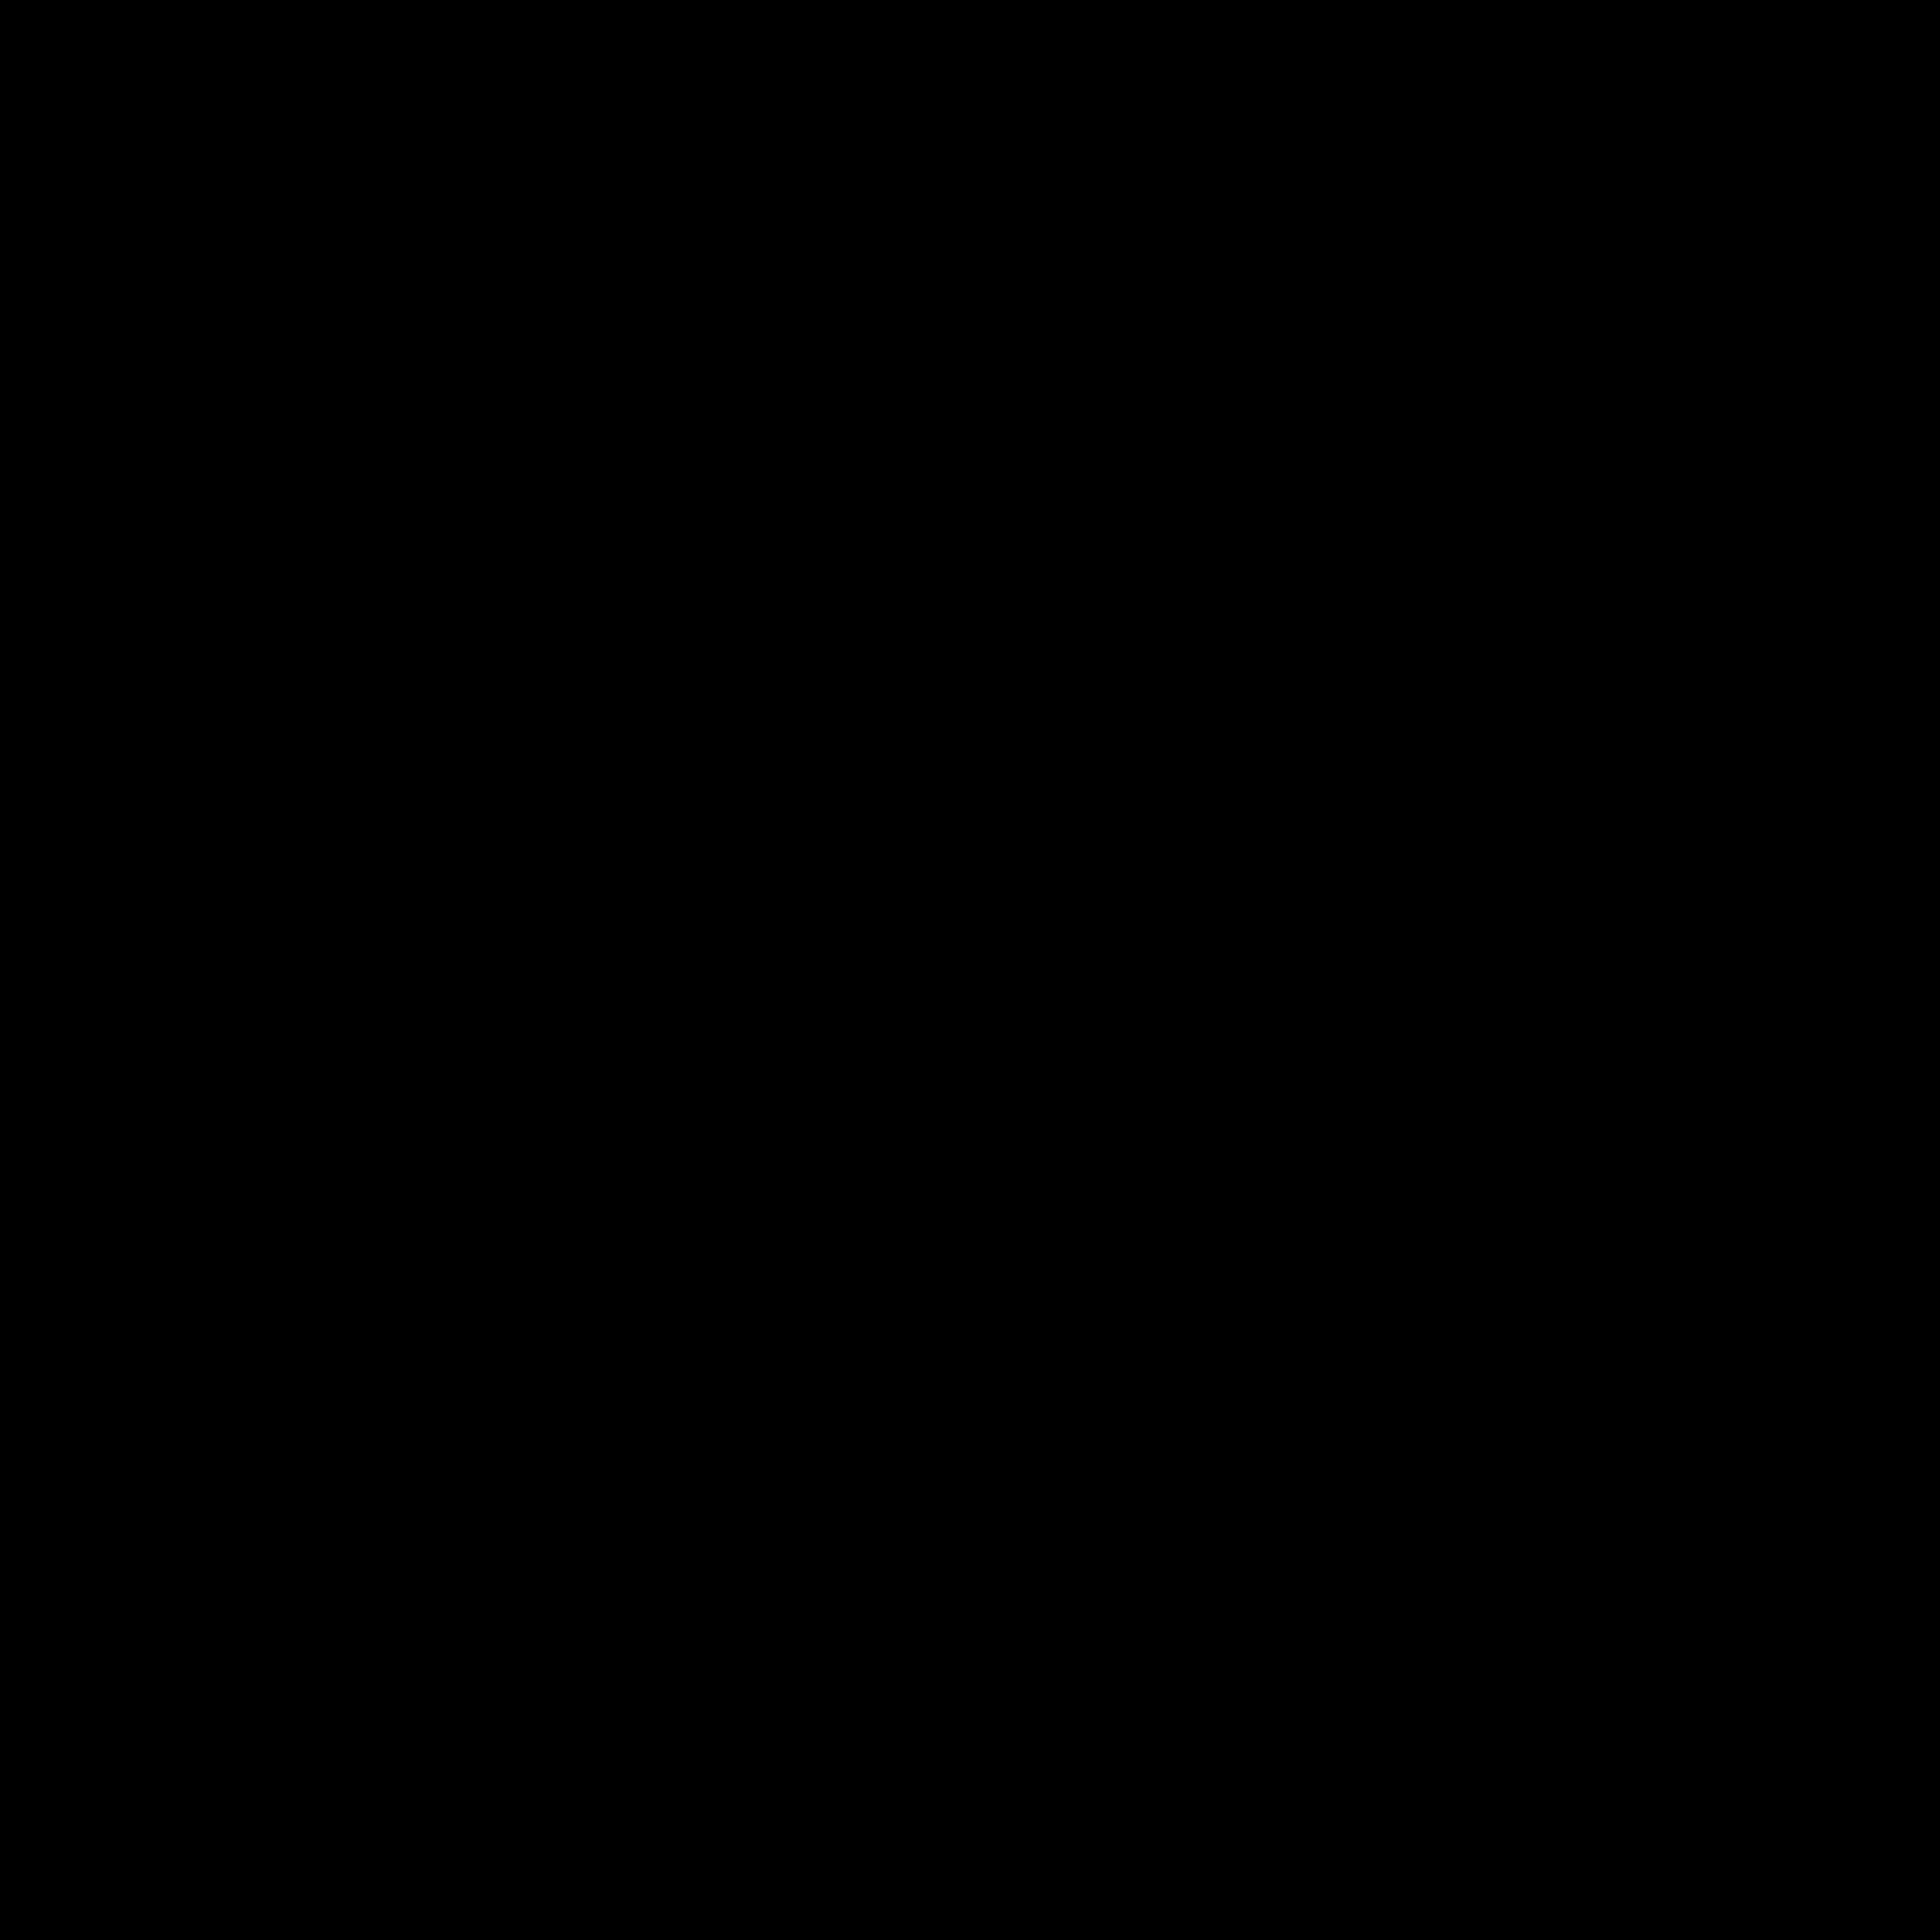
\includegraphics[width=\linewidth]{images/dense}
\caption{dense}
\end{subfigure}~%
\begin{subfigure}{\linewidth}
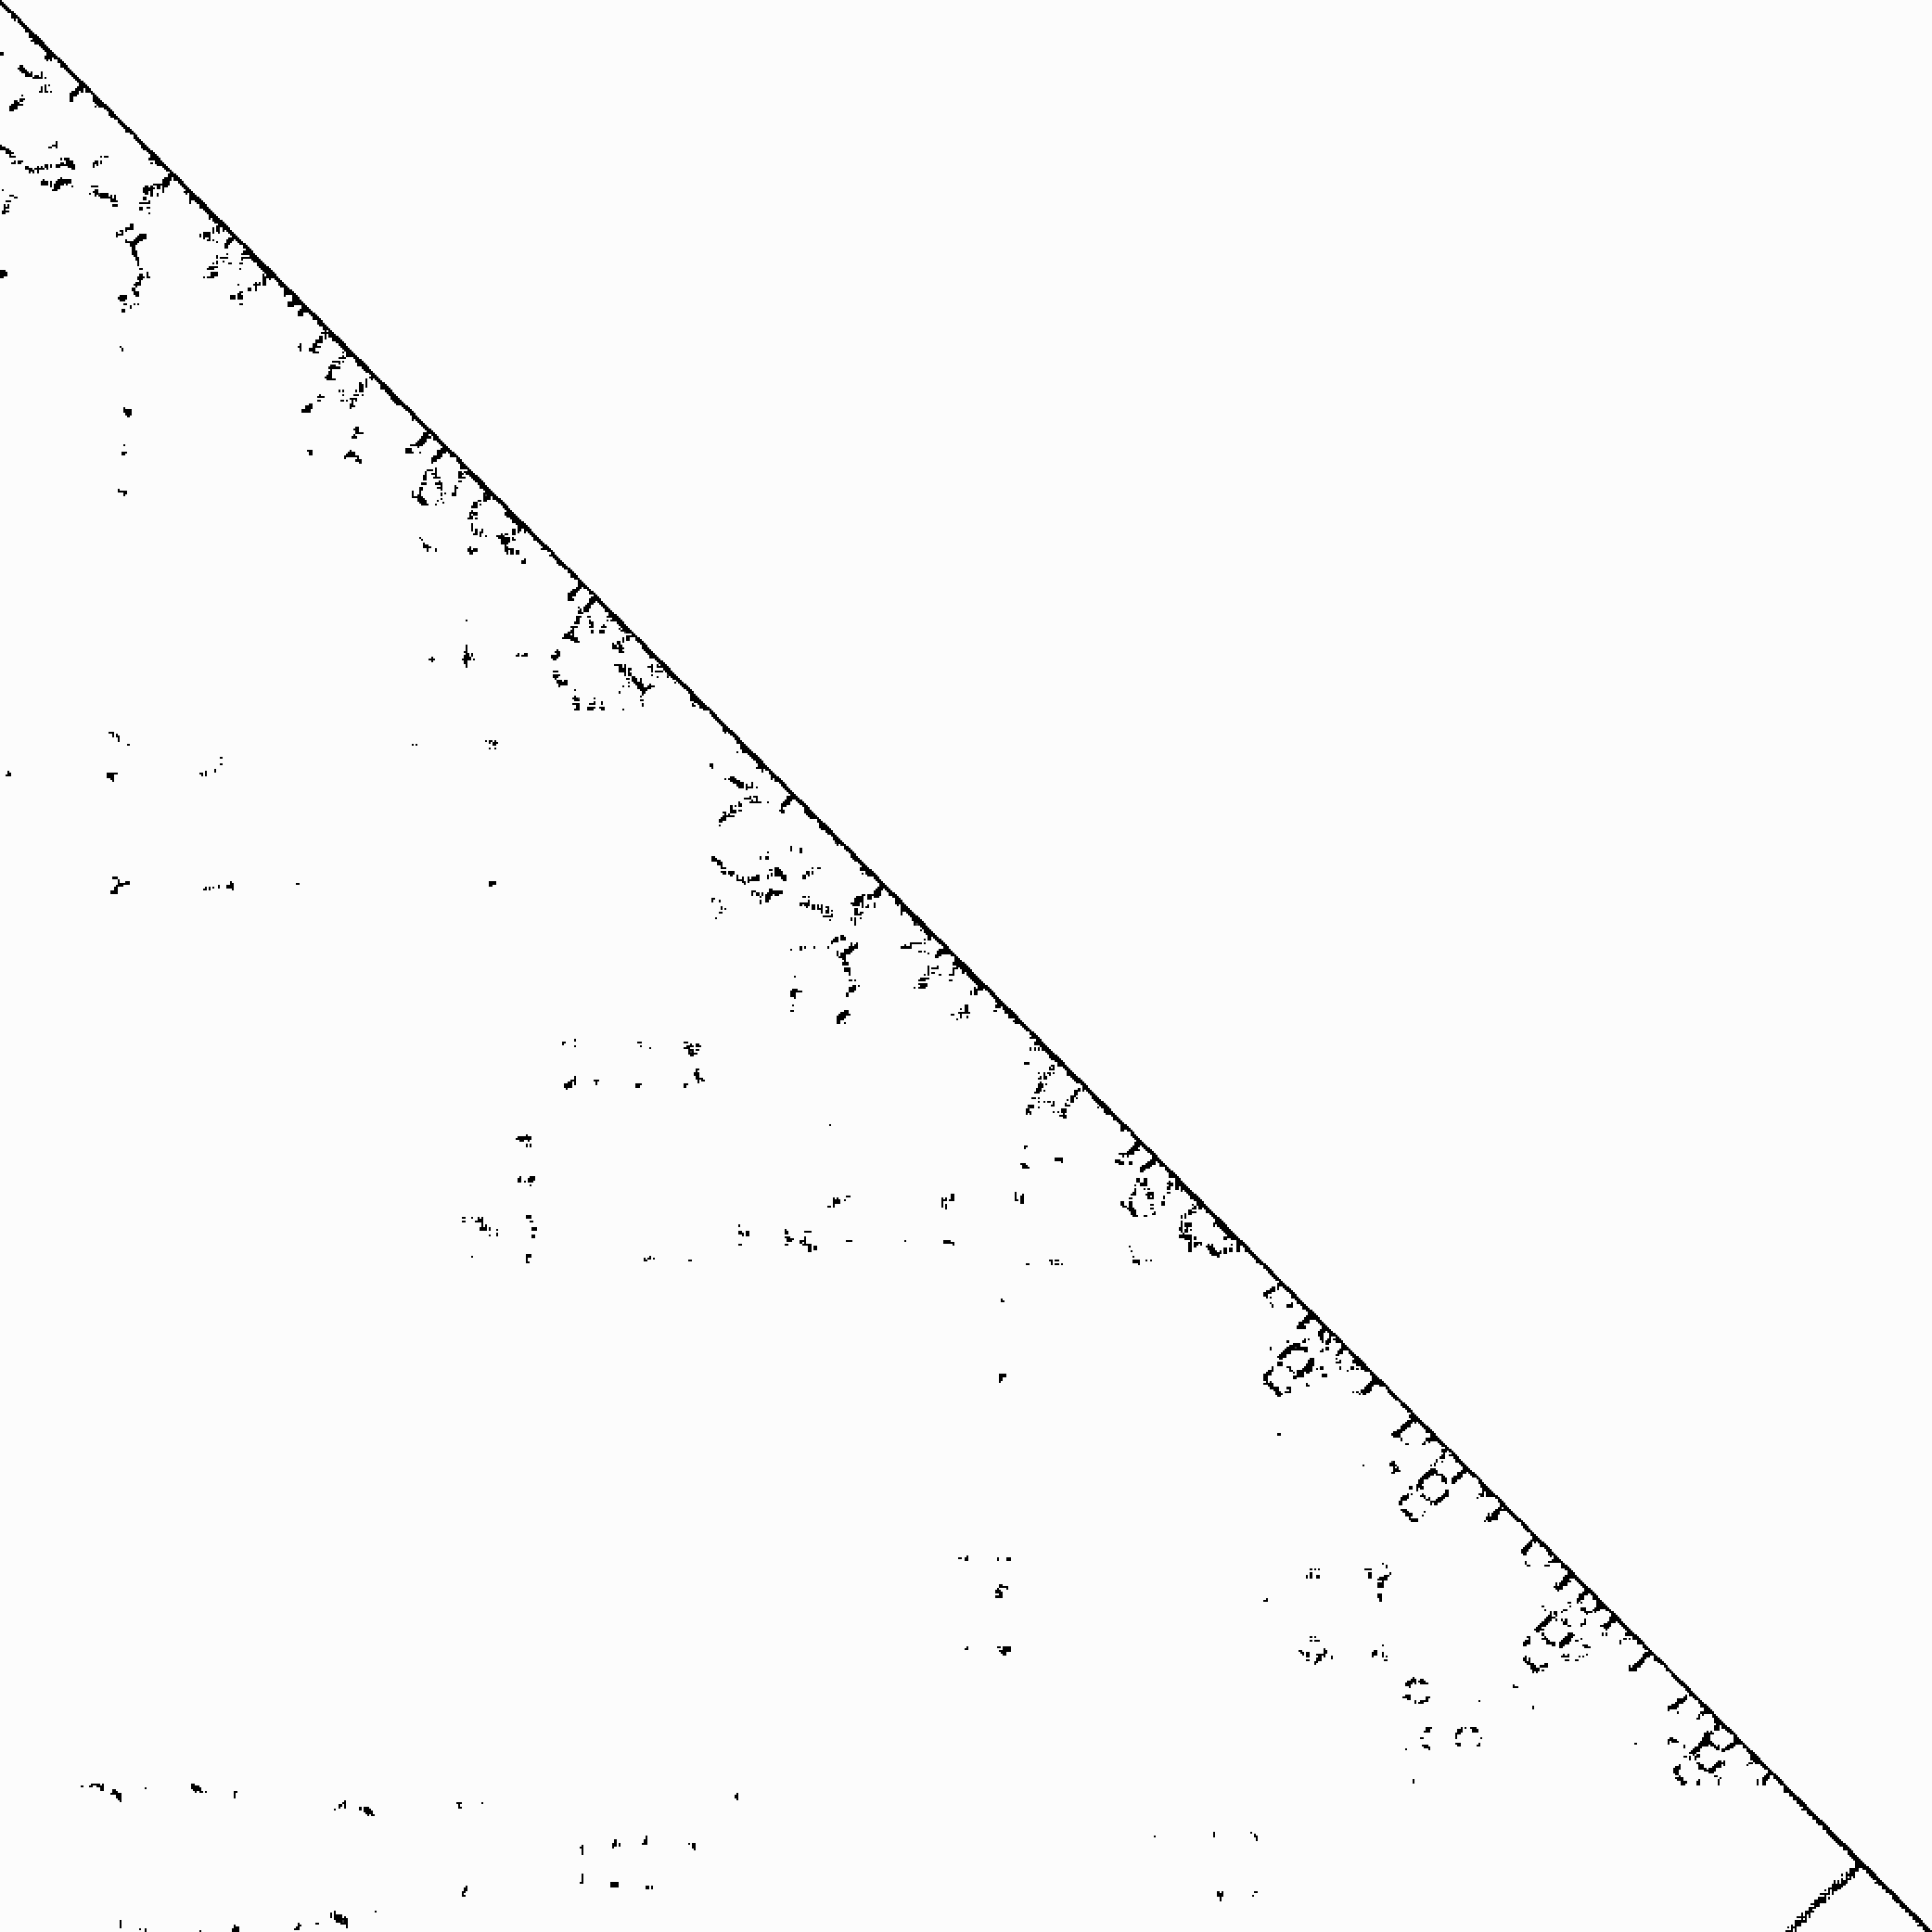
\includegraphics[width=\linewidth]{images/pdb1HYS}
\caption{pdb1HYS}
\end{subfigure}~%
\begin{subfigure}{\linewidth}
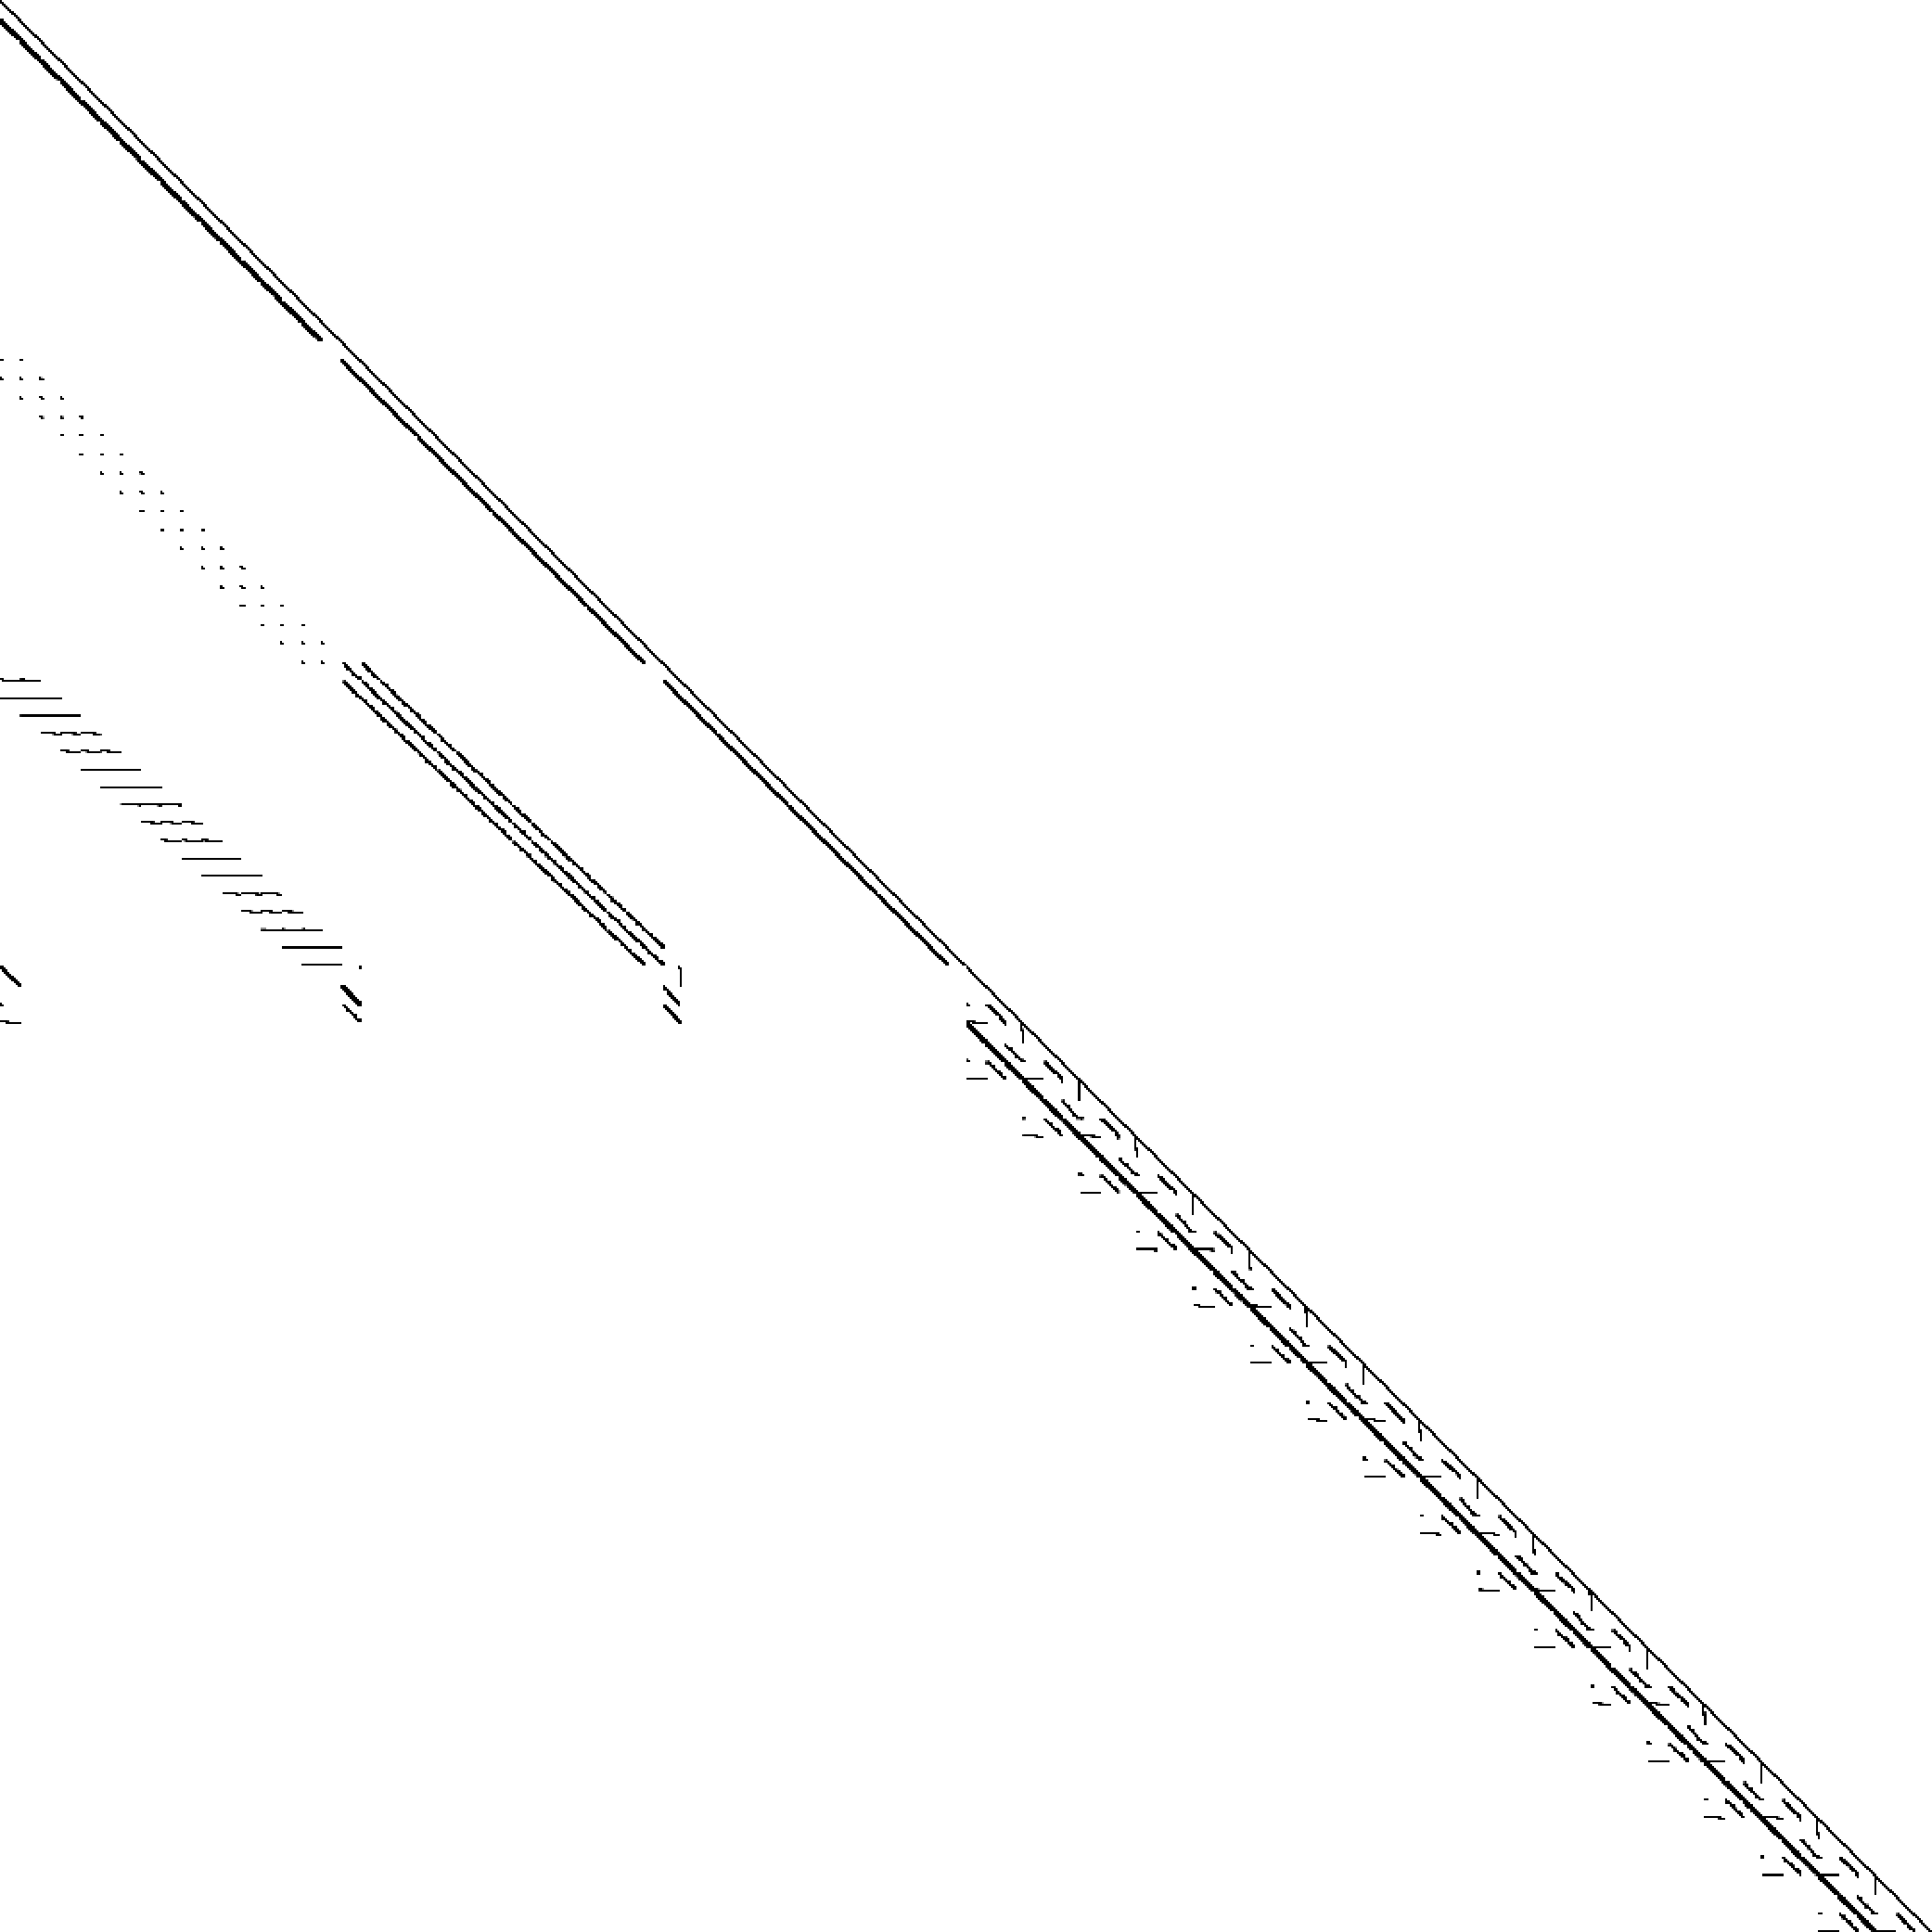
\includegraphics[width=\linewidth]{images/consph}
\caption{consph}
\end{subfigure}~%
\begin{subfigure}{\linewidth}
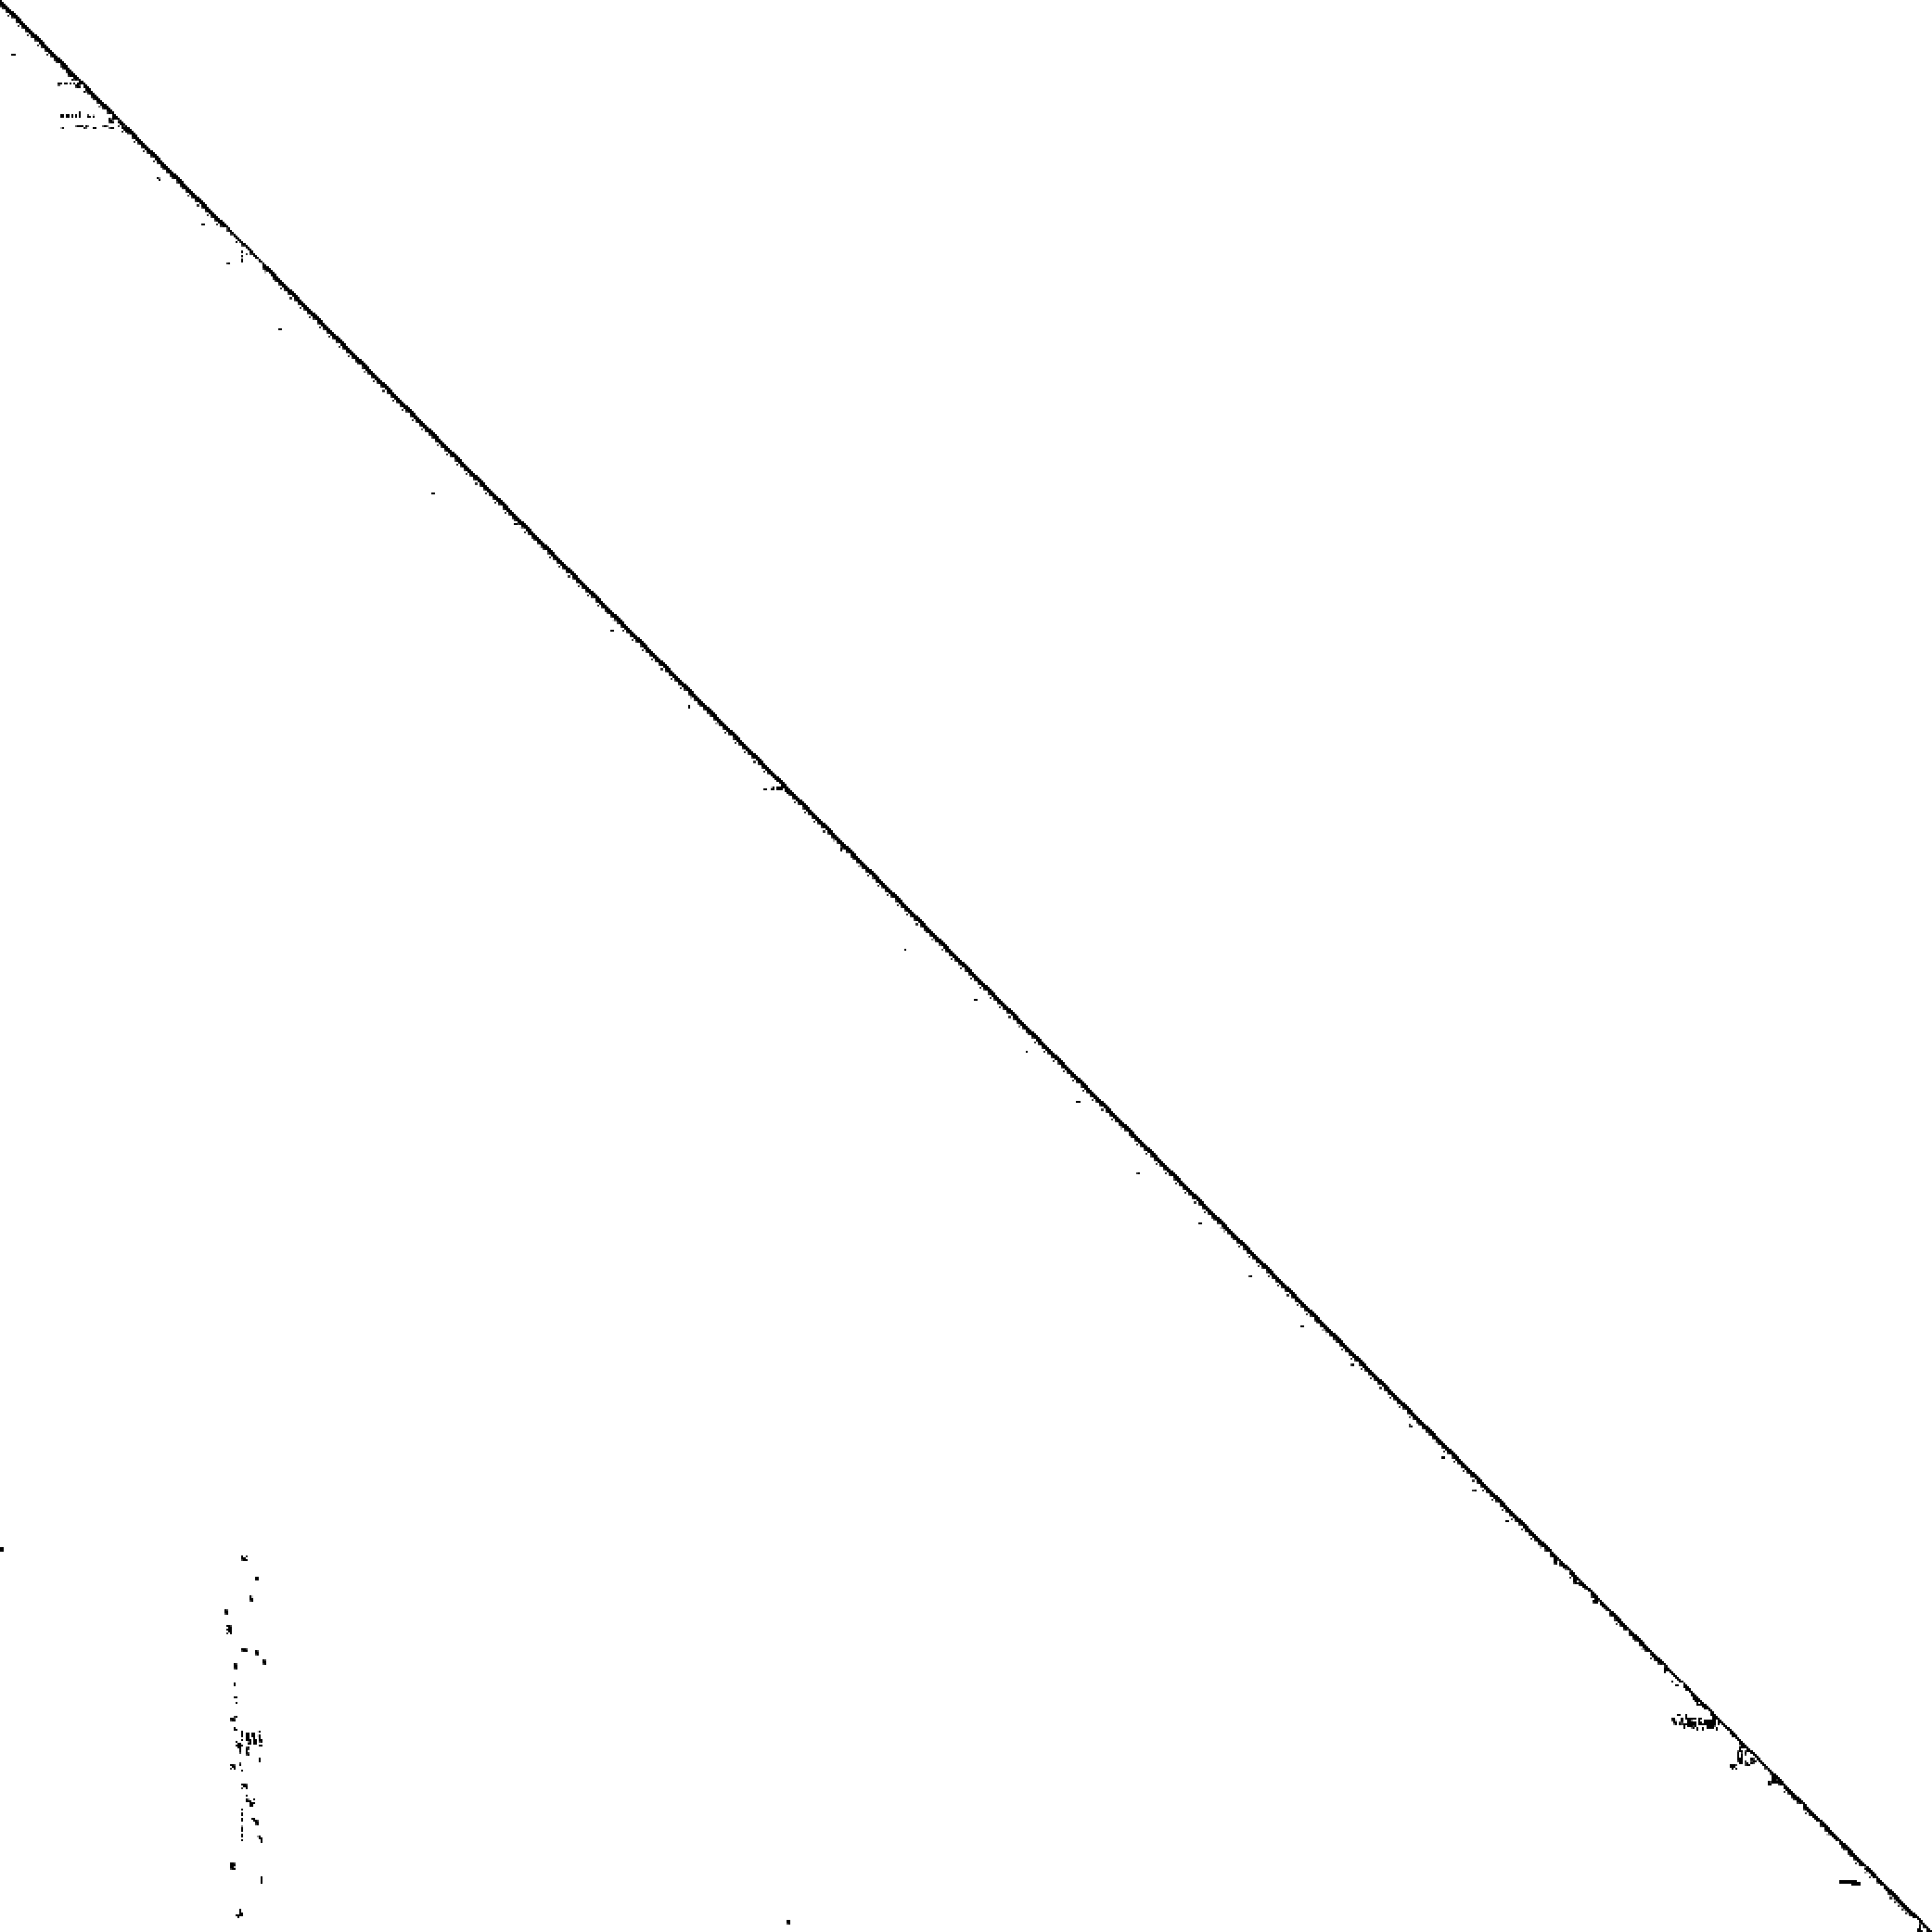
\includegraphics[width=\linewidth]{images/pwtk}
\caption{pwtk}
\end{subfigure}~%
\end{multicols}
\begin{multicols}{4}
\begin{subfigure}{\linewidth}
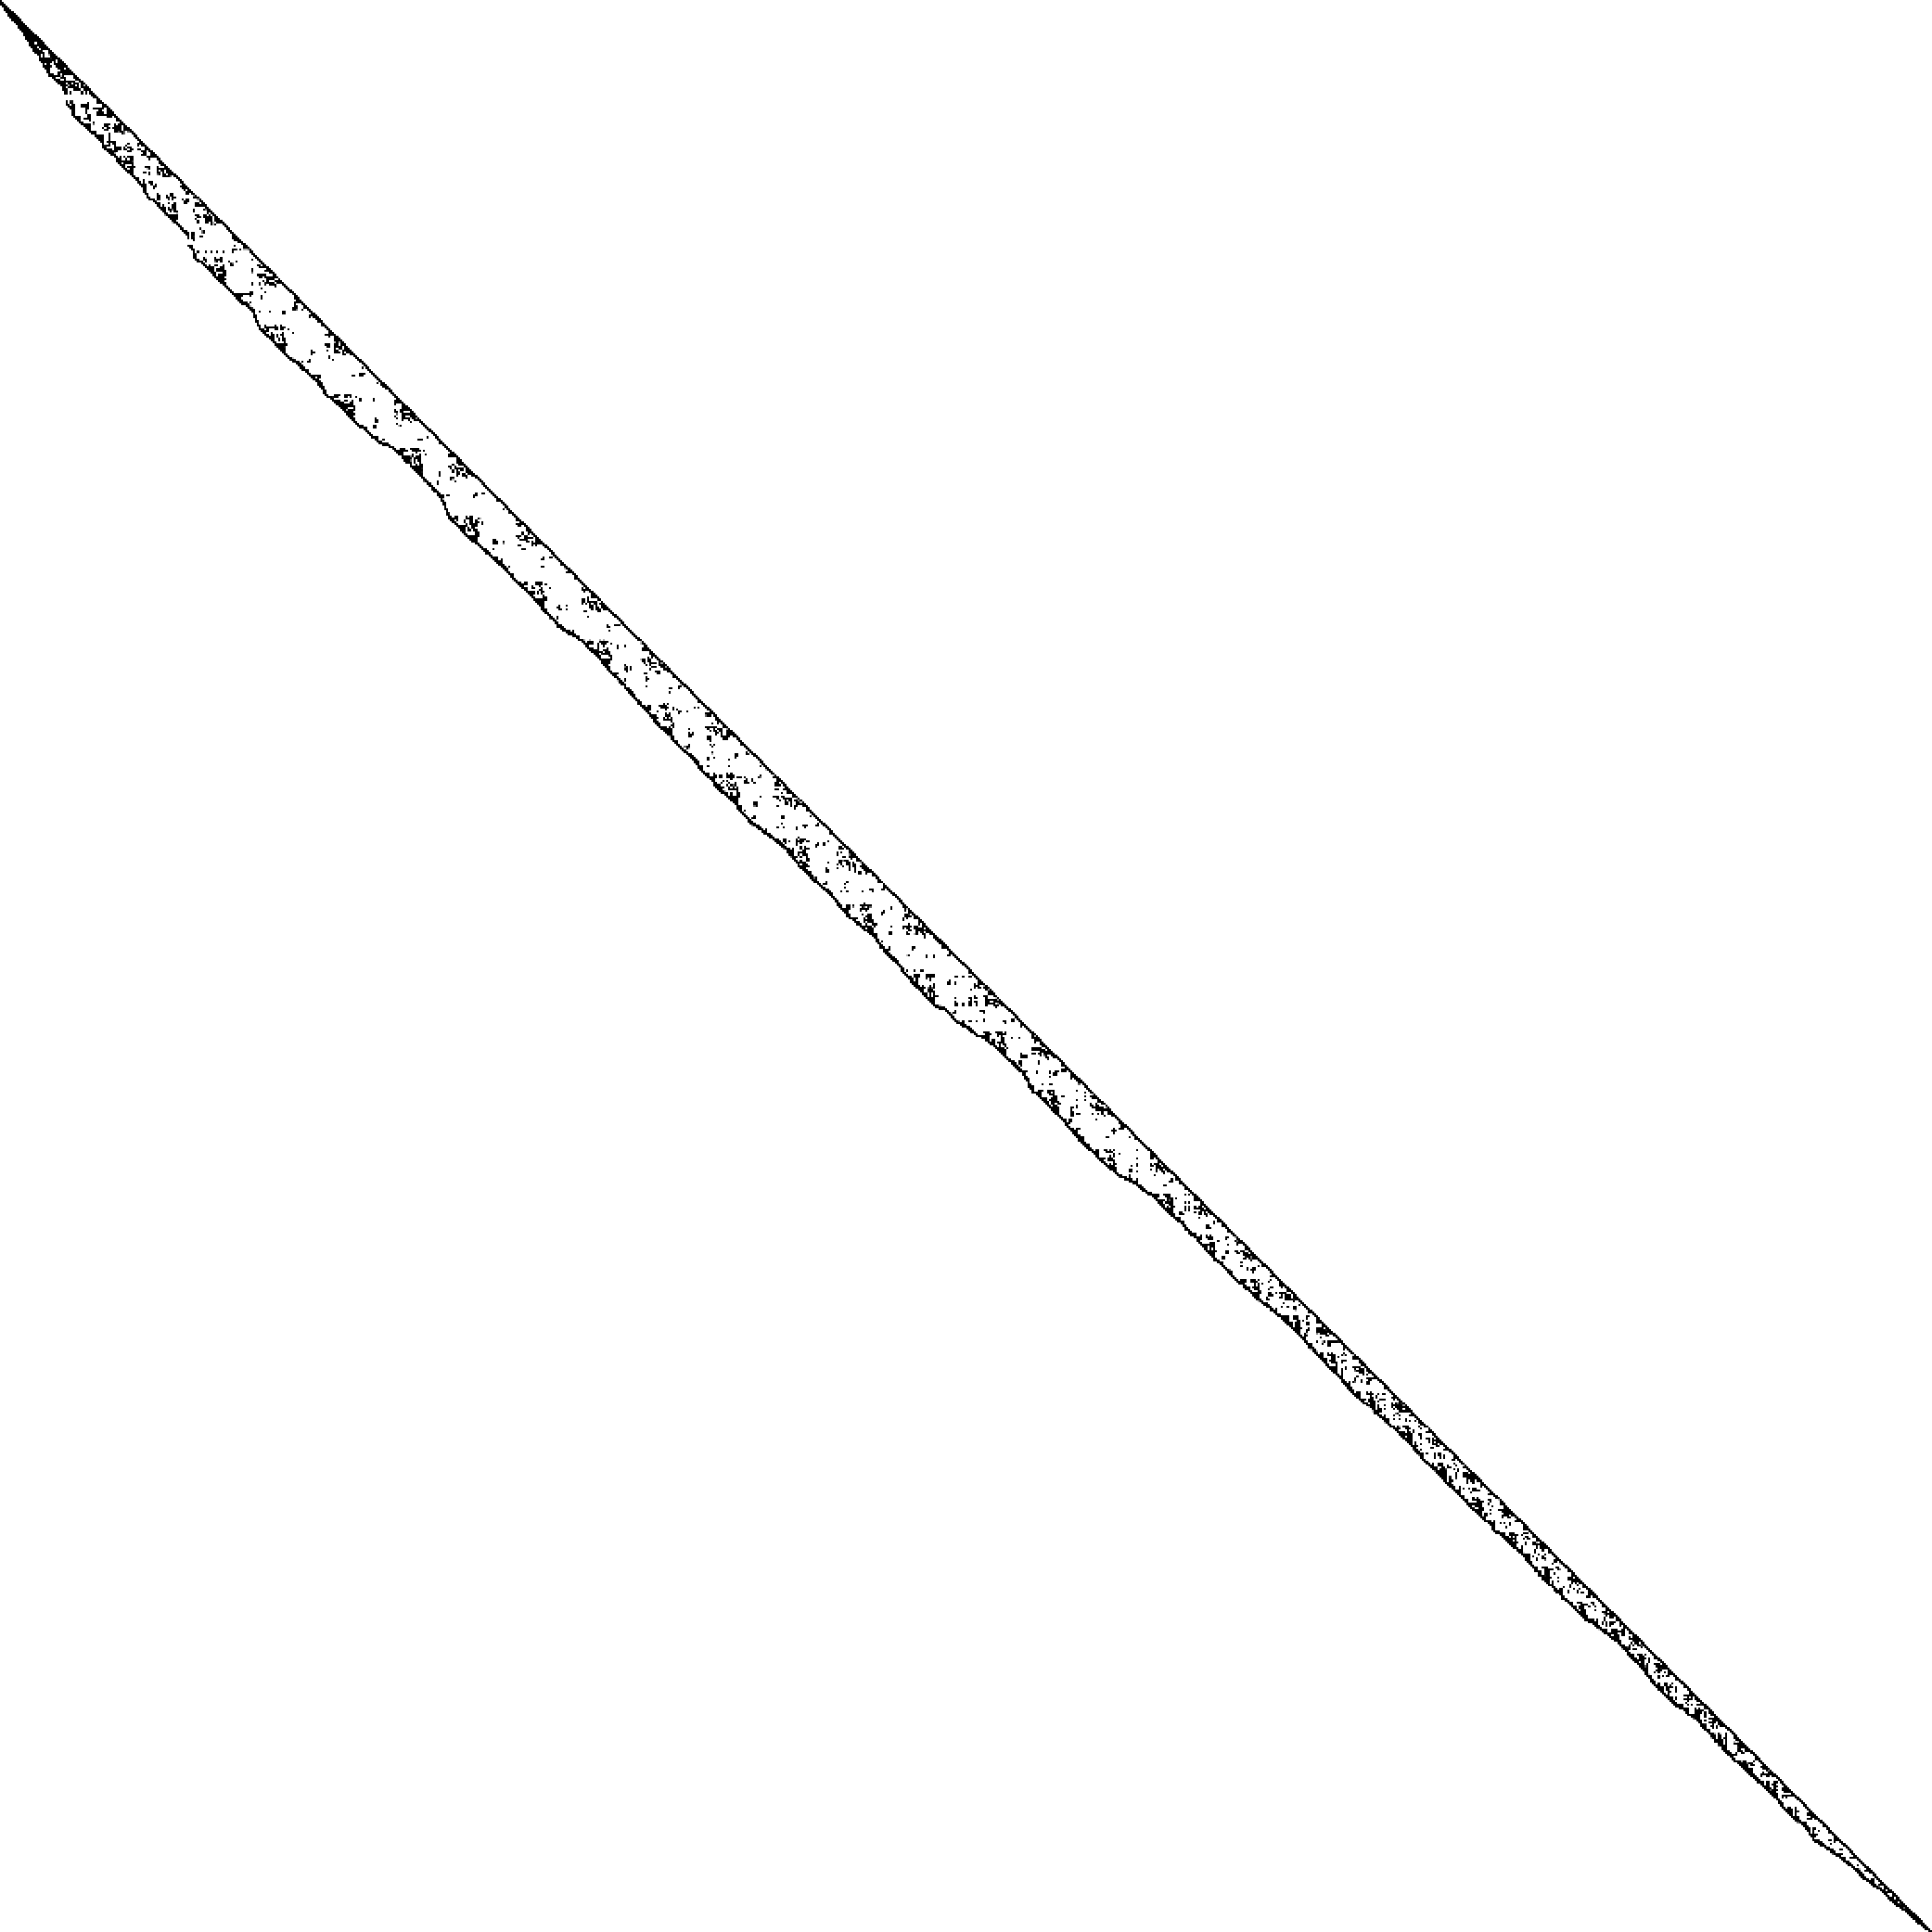
\includegraphics[width=\linewidth]{images/shipsec1}
\caption{shipsec1}
\end{subfigure}~%
\begin{subfigure}{\linewidth}

\includegraphics[width=\linewidth]{images/mac_econ_fwd500}
\caption{mac\_econ\_fwd500}
\end{subfigure}~%
\begin{subfigure}{\linewidth}
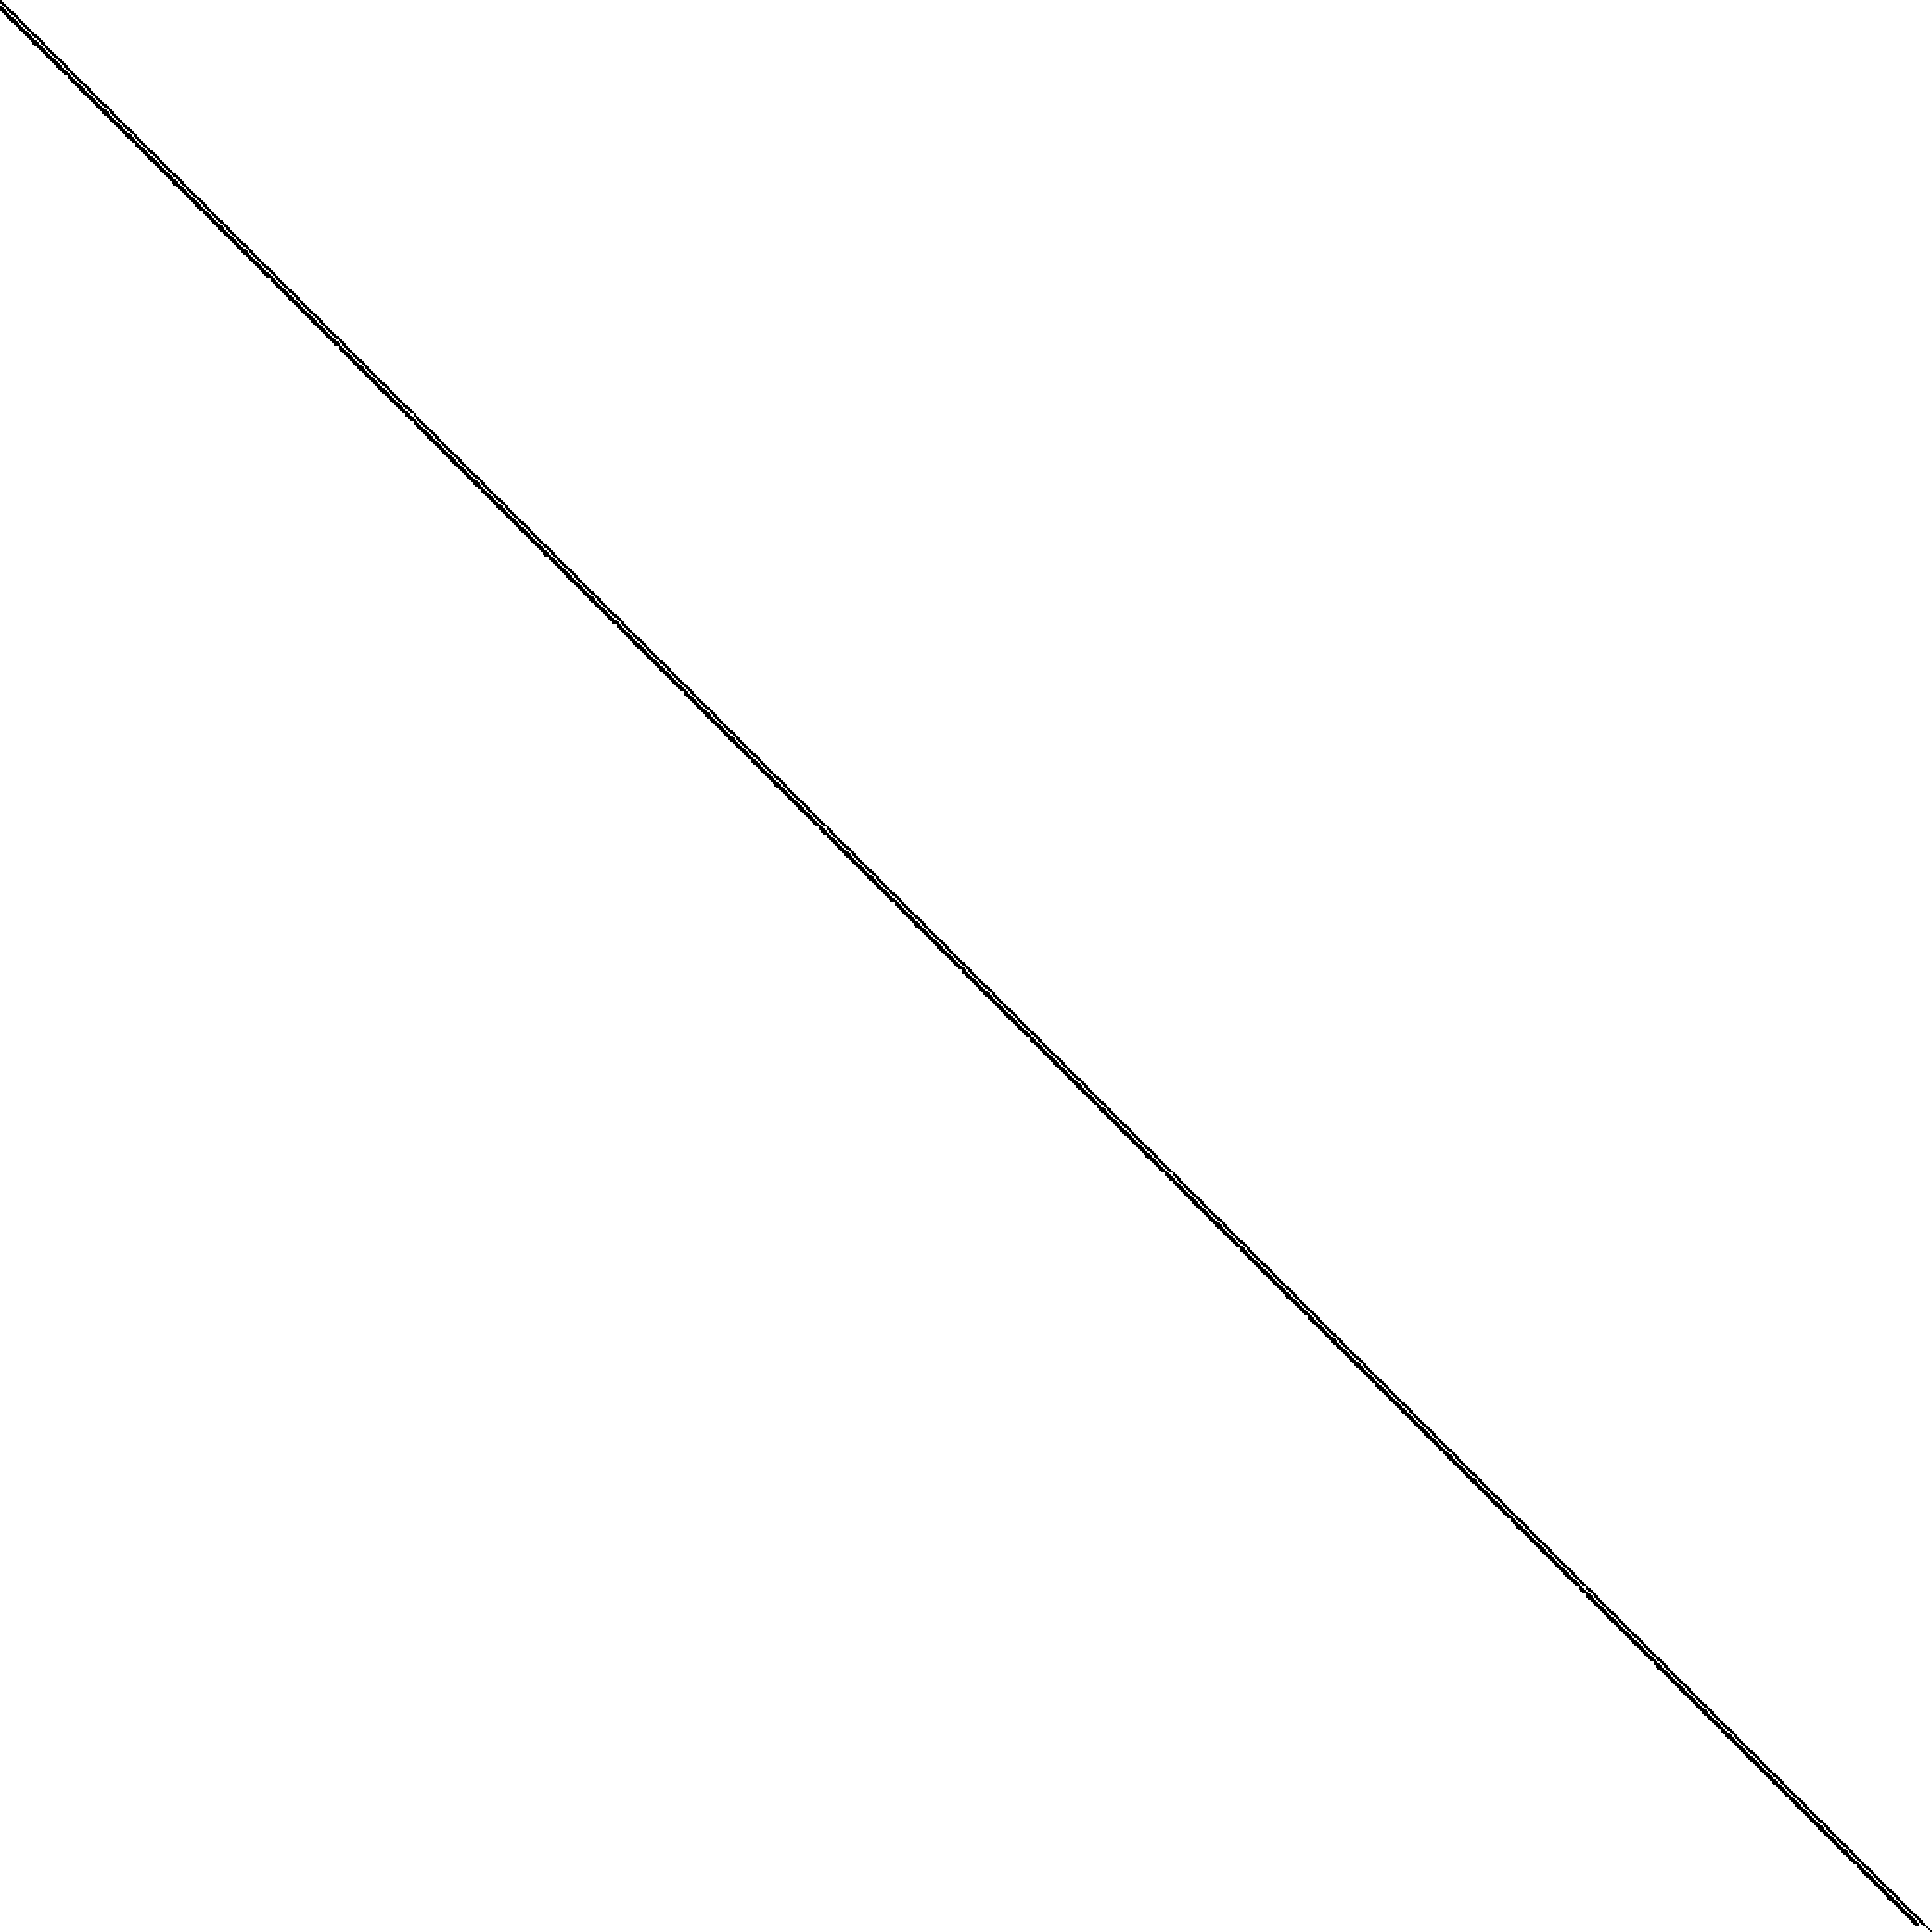
\includegraphics[width=\linewidth]{images/cant}
\caption{cant}
\end{subfigure}~%
\begin{subfigure}{\linewidth}
    
\includegraphics[width=\linewidth]{images/mc2depi}
    \caption{mc2depi}
\end{subfigure}
\end{multicols}
\begin{multicols}{4}
\begin{subfigure}{\linewidth}
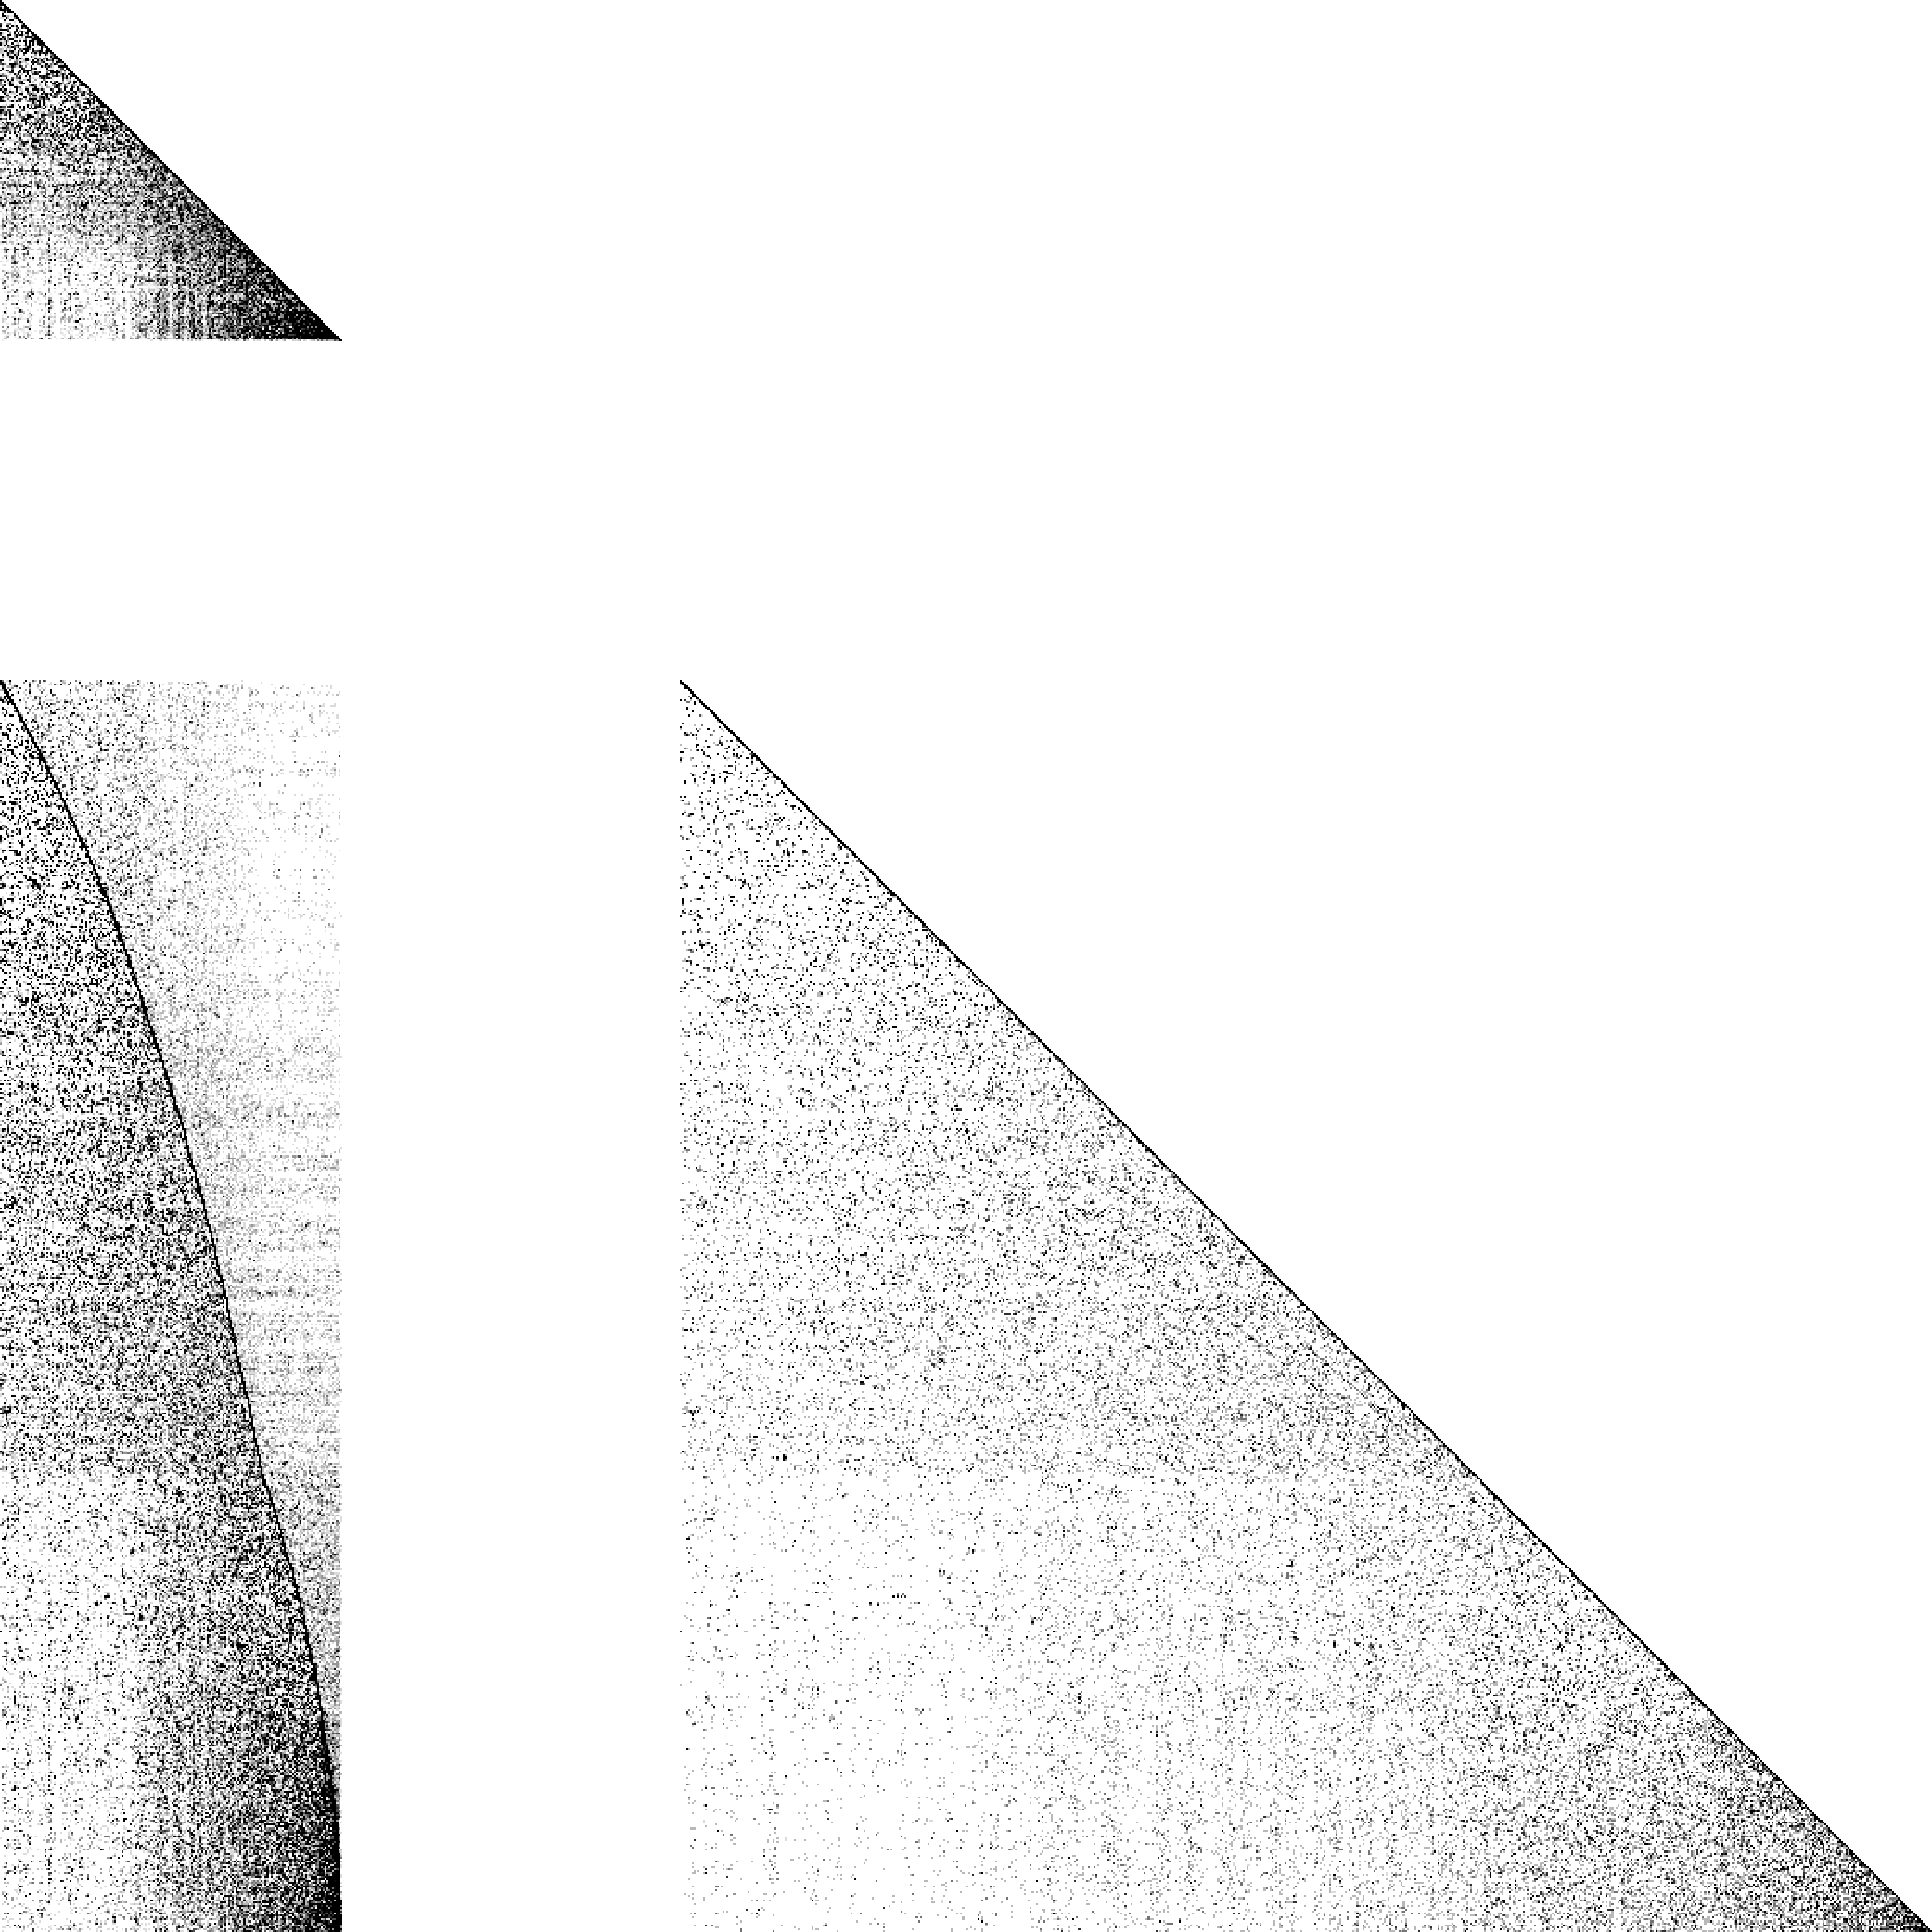
\includegraphics[width=\linewidth]{images/cop20k_A}
\caption{cop20k\_A}
\end{subfigure}~%
\begin{subfigure}{\linewidth}
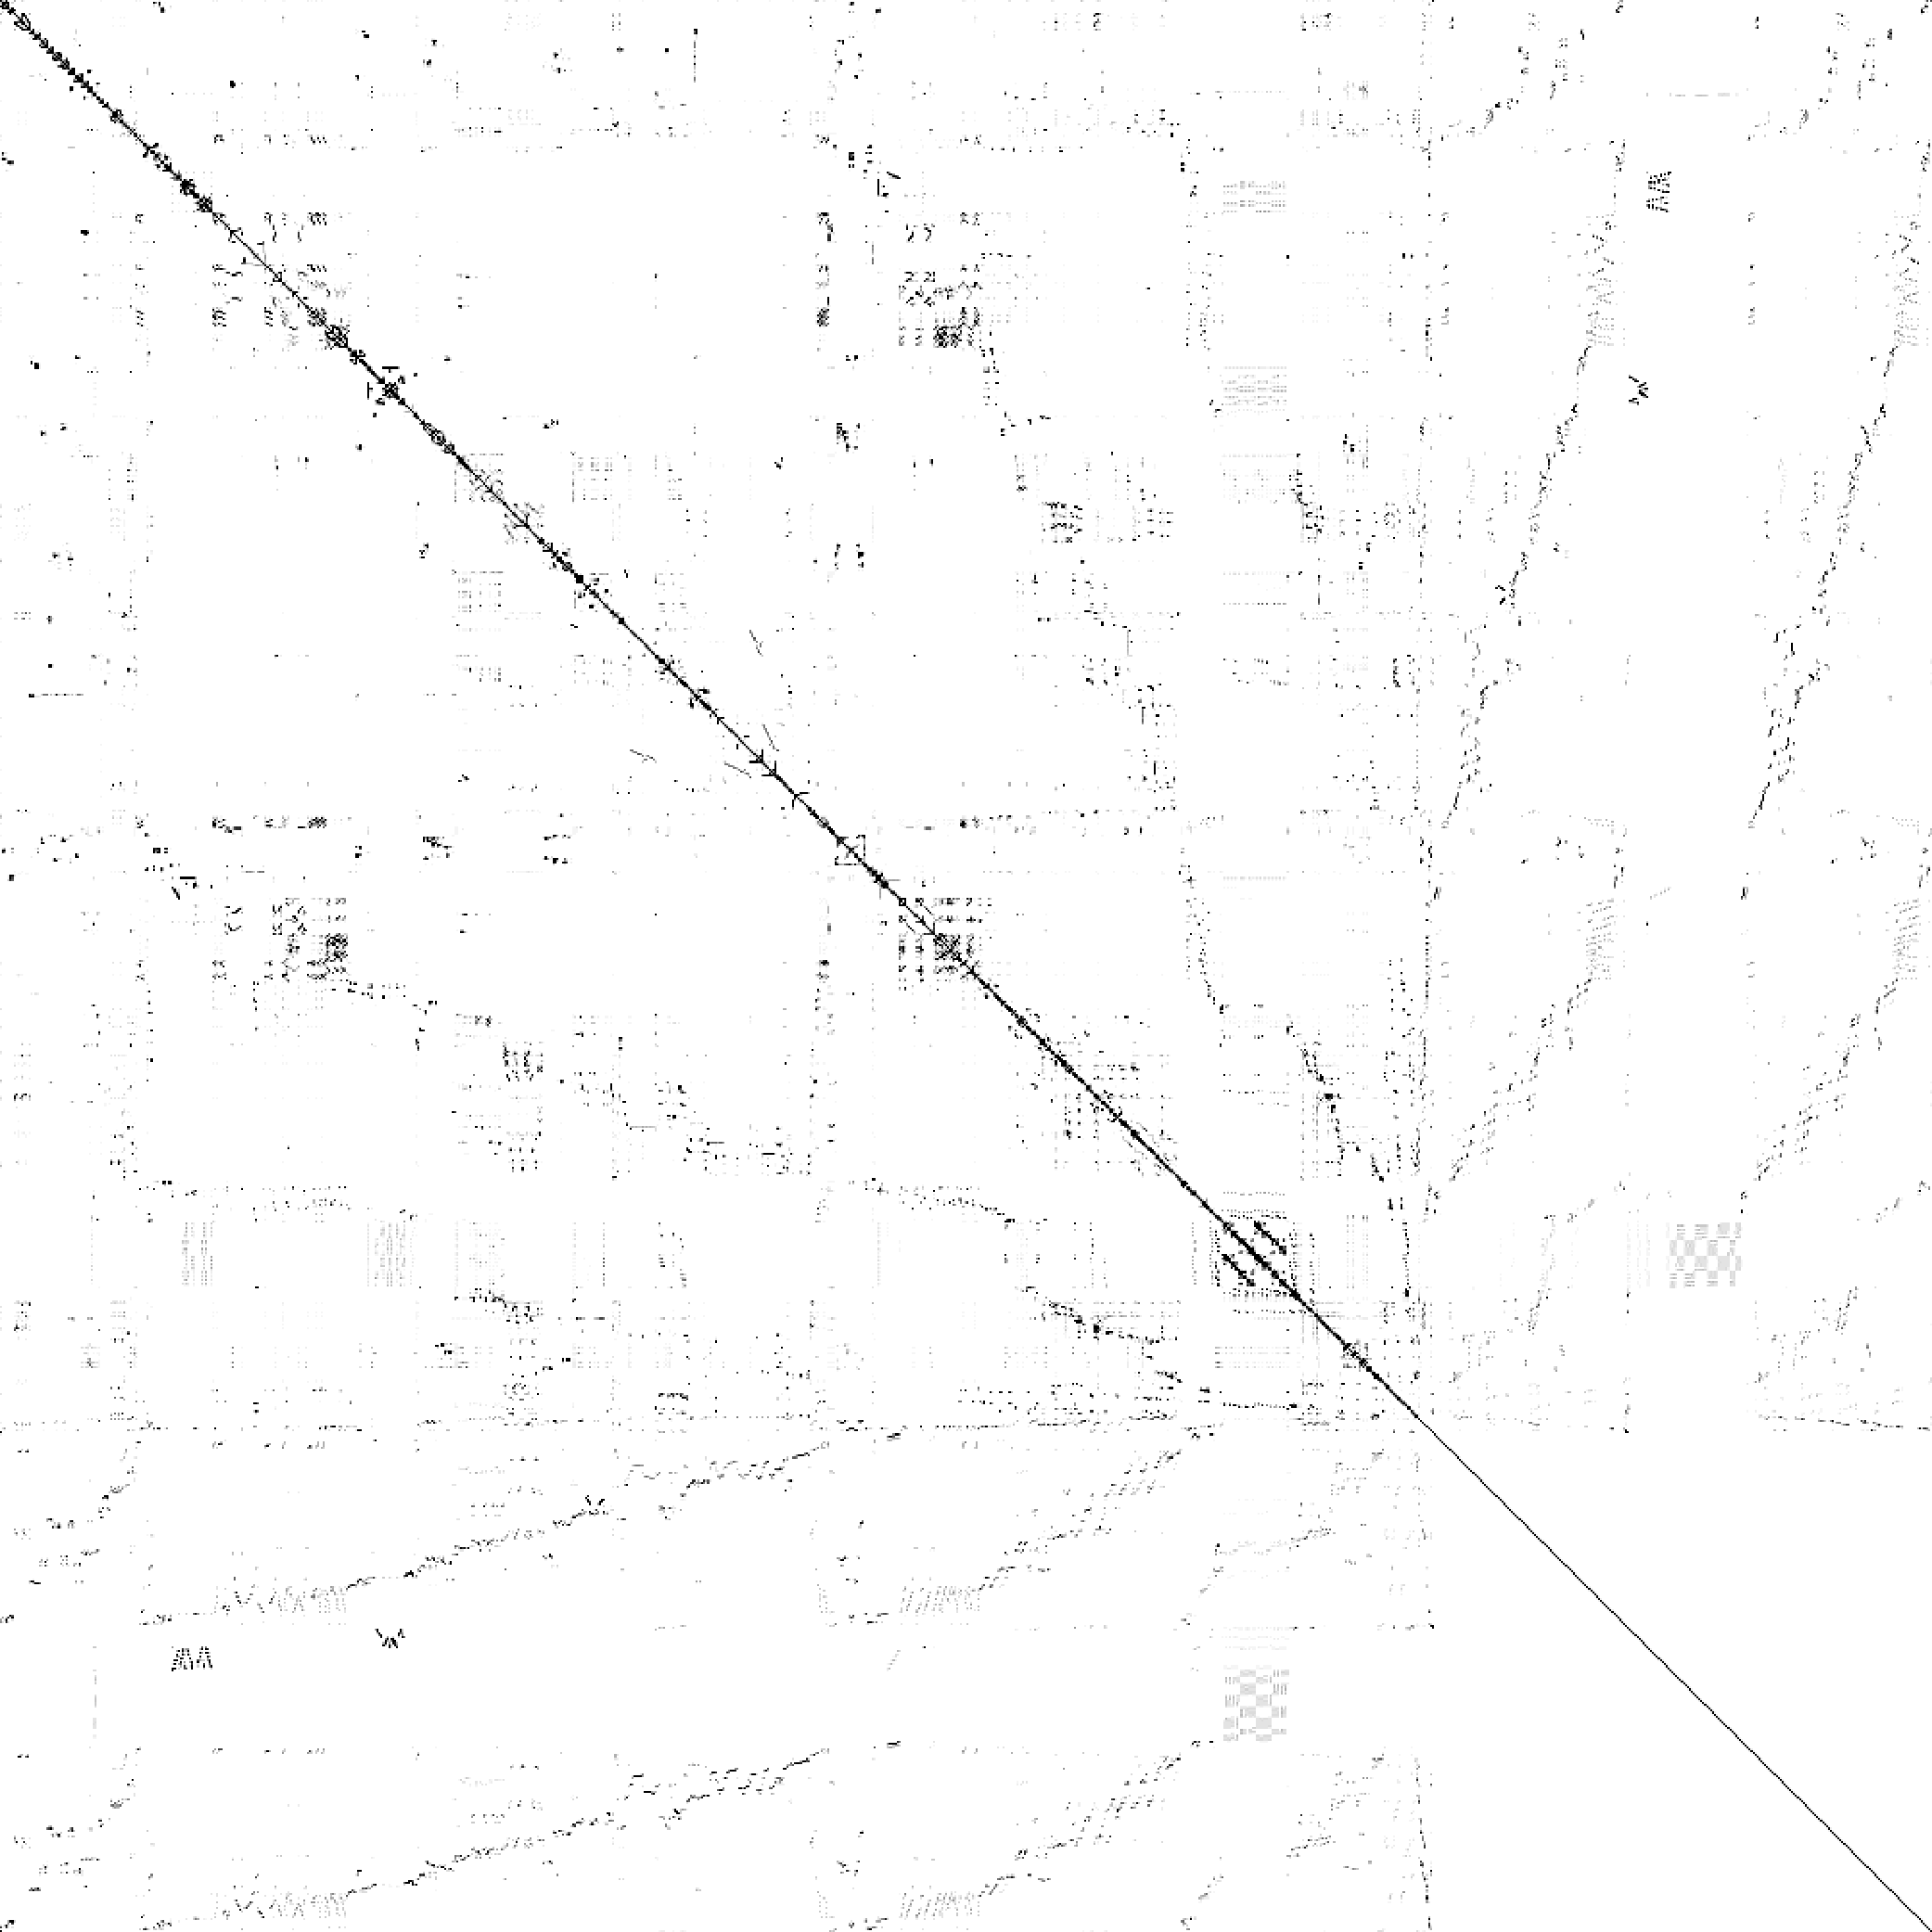
\includegraphics[width=\linewidth]{images/scircuit}
\caption{scircuit}
\end{subfigure}~%
\begin{subfigure}{\linewidth}
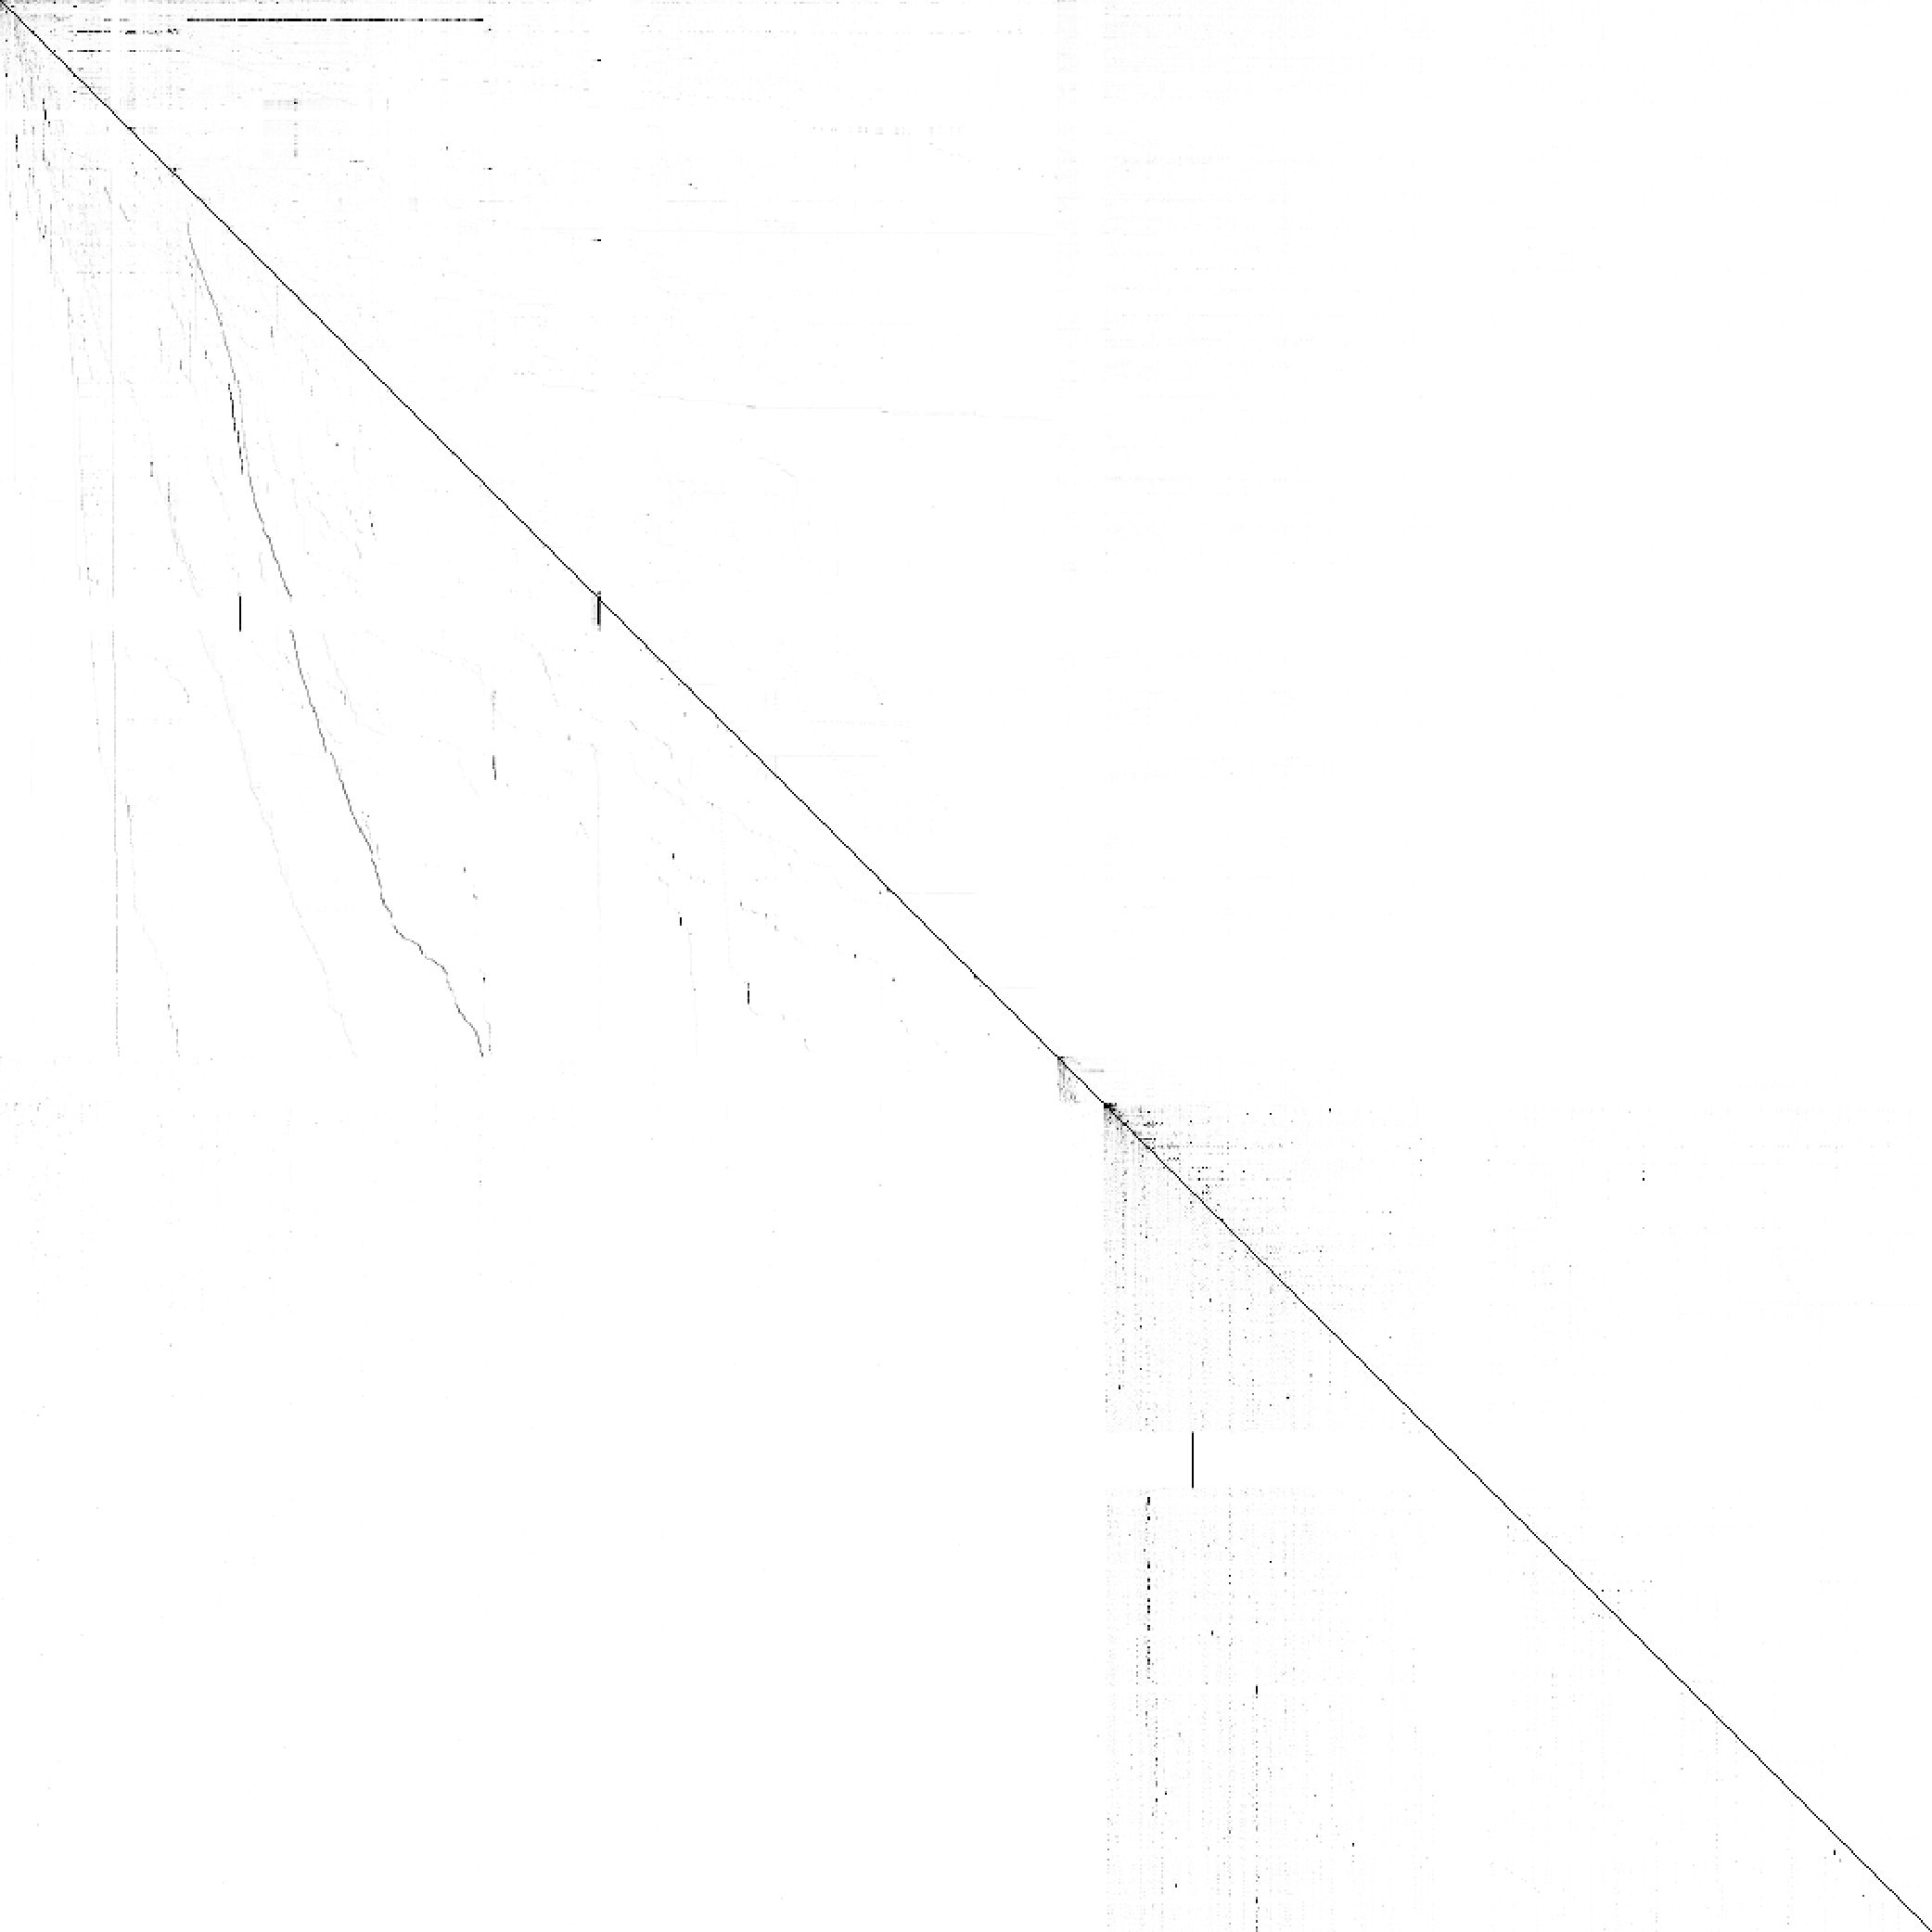
\includegraphics[width=\linewidth]{images/webbase-1M}
\caption{webbase-1M}
\end{subfigure}~%
\begin{subfigure}{\linewidth}
    \includegraphics[width=\linewidth]{images/qcd5_4}
    \caption{qcd5\_4}
\end{subfigure}
\end{multicols}
\begin{multicols}{4}
\begin{subfigure}{\linewidth}
    \includegraphics[width=\linewidth]{images/rma10}
    \caption{rma10}
\end{subfigure}~%
\begin{subfigure}{\linewidth}
    \includegraphics[width=\linewidth]{images/rail4284}
    \caption{rail4284}
\end{subfigure}
\end{multicols}

\caption[Matrices]{The density plots of the matrices used for testing}
\label{fig:matrices}
\end{figure}
OK, now that we have a good background about SpMV, the platforms it can run on and optimizations for SpMV, we need a way to determine which implementation performs the best. This is where benchmarking comes in. However, different matrices can have vastly different SpMV performance. So a test set of matrices is used (\figurename~\ref{fig:matrices}). In \figurename~\ref{fig:nnzVgflops} we show the performance of SpMV on CPUs, GPUs and FPGAs. As you can see the performance is very jumpy from matrix to matrix. Three factors effect the performance: dimension, sparsity, and values. \par
\begin{figure*}
\centering
\begin{tikzpicture}[scale=1]

 \ifthenelse{\equal{\blackandwhite}{true}}{
	\tikzstyle{yellowStar}=[draw, diamond, fill=black!65, inner sep =1.5pt];
	\tikzstyle{blueGreenDiamond}=[draw, diamond, fill=black!75, inner sep =1.5pt];
	\tikzstyle{greenSquare}=[draw, rectangle, fill=black!50, inner sep =2.5pt];
	\tikzstyle{blueTriangle}=[draw, regular polygon, regular polygon sides=3, fill=black!35, inner sep =1.5pt];
 }{
	\tikzstyle{yellowStar}=[draw, star, star points=5, fill=yellow, inner sep =1.5pt];
	\tikzstyle{blueGreenDiamond}=[draw, diamond, fill=green!60!blue, inner sep =1.5pt];
	\tikzstyle{greenSquare}=[draw, rectangle, fill=green, inner sep =2.5pt];
	\tikzstyle{blueTriangle}=[draw, regular polygon, regular polygon sides=3, fill=blue, inner sep =1.5pt];
 }

%\draw [ystep=2.0,gray,very thin, xstep = 14] (0,0) grid (12.9, 6.9);
\draw [->,thick] (0,0) to (14.5, 0);
\draw [->, thick] (0,0) to (0,7);
\foreach \x/\mat/\size in { %
0/dw8192/42K, 1/t2d\_q9/87K, 2/epb1/95K, 3/raefsky1/290K, 4/psmigr\_2/540K, 6/torso2/1M%
}
	\draw (\x cm, 1pt) -- (\x cm, -1pt) node[anchor=east,rotate=90,gray] {\shortstack{\mat (\size)}};
\foreach \x/\mat/\size in { %
5/scircuit/960K, 7/mac\_econ/1.3M, 8/qcd5\_4/1.9M, 9/mc2depi/2.1M, 10/rma10/2.3M, 11/shipsec1/3.6M, 12/dense/4M, 13/cant/4M, 14/consph/6M%
}
	\draw (\x cm, 1pt) -- (\x cm, -1pt) node[anchor=east,rotate=90] {\shortstack{\mat (\size)}};
\foreach \y/\ytext in {0/0,1/5,2/10, 3/15, 4/20, 5/25, 6/30}
	\draw (1pt, \y cm) -- (-1pt, \y cm) node[anchor=east] {$\ytext$};
%\node at (6, -.8) {Size of Matrix (Millions)};
\node at (-1, 3) [rotate=90]{Performance (Gflops)};

%R3 line
\foreach \i/\j/\k/\l in {%
0/0.42000000000000004/1/0.76,  1/0.76/2/0.6599999999999999,  2/0.6599999999999999/3/1.04,  3/1.04/4/0.9800000000000001,  4/0.9800000000000001/5/1.24,  5/1.24/6/1.28,  6/1.28/7/1.1800000000000002,  7/1.1800000000000002/8/2.56,  8/2.56/9/1.24,  9/1.24/10/2.7199999999999998,  10/2.7199999999999998/11/1.58,  11/1.58/12/2.7199999999999998,  12/2.7199999999999998/13/2.54,  13/2.54/14/1.7399999999999998
}{
 \ifthenelse{\equal{\blackandwhite}{true}}{
	\draw [black] (\i,\j) -- (\k,\l);
 }{
	\draw [red] (\i,\j) -- (\k,\l);
 }
}

%hc1 line
\foreach \i/\j/\k/\l in {%
0/0.33999999999999997/1/0.5,  1/0.5/2/0.52,  2/0.52/3/0.78,  3/0.78/4/0.78,  4/0.78/6/0.24
}{
 \ifthenelse{\equal{\blackandwhite}{true}}{
	\draw [black!65] (\i,\j) -- (\k,\l);
 }{
	\draw [brown] (\i,\j) -- (\k,\l);
 }
}

%%tesla line
%\foreach \i/\j/\k/\l in {%
%0/0.1/1/0.18,  1/0.18/2/0.16,  2/0.16/3/0.5599999999999999,  3/0.5599/5/0.6}
%	\draw <3,5>[green!60!blue] (\i,\j) -- (\k,\l);

%m2090 line
\foreach \i/\j/\k/\l in {%
5/1.2/7/1.2,  7/1.2/8/4.0,  8/4.0/9/4.4,  9/4.4/10/2.2,  10/2.2/11/2.2,  11/2.2/12/4.6,  12/4.6/13/3.4,  13/3.4/14/3.0
}{
 \ifthenelse{\equal{\blackandwhite}{true}}{
	\draw [black!50] (\i,\j) -- (\k,\l);
 }{
	\draw [green] (\i,\j) -- (\k,\l);
 }
}

%intel line
\foreach \i/\j/\k/\l in {%
5/2.4/7/4.6,  7/4.6/8/6.0,  8/6.0/9/4.2,  9/4.2/10/4.8,  10/4.8/11/2.0,  11/2.0/12/2.8,  12/2.8/13/2.4,  13/2.4/14/2.2
}{
 \ifthenelse{\equal{\blackandwhite}{true}}{
	\draw [black!35] (\i,\j) -- (\k,\l);
 }{
	\draw [blue] (\i,\j) -- (\k,\l);
 }
}


\draw [dashed] (.5, -.5) -- (.5, 7) node [fill=white,inner sep=0pt, midway,below, sloped]{\small $(64K)$};

\draw [dashed] (10.5, -.5) -- (10.5, 7)  node [fill=white,inner sep=0pt, near end,below, sloped]{\small 20MB $(2.5M)$};



%hc1 points
\foreach \i/\x/\y/\f/\q/\u in {%
0/0.083492/0.33999999999999997/1.7/0/-.2,%
1/0.17405/0.5/2.5/0/-.1,%
2/0.190106/0.52/2.6/0/-.2,%
3/0.588552/0.78/3.9/0/-.2,%
4/1.080044/0.78/3.9/0/-.2,%
6/2.066946/0.24/1.2/0/0
}{
 \ifthenelse{\equal{\blackandwhite}{true}}{
	\draw (\i,\y) node[yellowStar]{} node[fill=white,inner sep=0pt, anchor=west,rotate=30,xshift=\q cm + 3pt, yshift=\u cm] {\color{black!65} \scriptsize $\f$};
 }{
	\draw (\i,\y) node[yellowStar]{} node[fill=white,inner sep=0pt, anchor=west,rotate=30,xshift=\q cm + 3pt, yshift=\u cm] {\color{brown} \scriptsize $\f$};
 }
}	

%intel points
\foreach \i/\x/\y/\f/\q/\u in {%
5/1.917872/2.4/12/0/0,%
7/2.546778/4.6/23/0/0,%
8/3.833856/6.0/30/0/0,%
9/4.20045/4.2/21/0/-.2,%
10/4.658184/4.8/24/0/0,%
11/7.136352/2.0/10/0/0,%
12/8.0/2.8/14/0/.2,%
13/8.014766/2.4/12/0/-.2,%
14/12.02096/2.2/11/0/0
}{
 \ifthenelse{\equal{\blackandwhite}{true}}{
	\draw (\i cm,\y cm) node[blueTriangle]{} node[fill=white,inner sep=0pt, anchor=west,rotate=30,xshift=\q cm + 3pt, yshift=\u cm]{\color{black!50} \scriptsize $\f$};
 }{
	\draw (\i cm,\y cm) node[blueTriangle]{} node[fill=white,inner sep=0pt, anchor=west,rotate=30,xshift=\q cm + 3pt, yshift=\u cm]{\color{blue} \scriptsize $\f$};
 }
}

%M2090 points
\foreach \i/\x/\y/\f/\q/\u in {%
5/1.917872/1.2/6/0/-.3,%
7/2.546778/1.2/6/0/.3,%
8/3.833856/4.0/20/0/0,%
9/4.20045/4.4/22/0/0,%
10/4.658184/2.2/11/0/0,%
11/7.136352/2.2/11/0/.1,%
12/8.0/4.6/23/0/0,%
13/8.014766/3.4/17/0/0,%
14/12.02096/3.0/15/0/0
}{
 \ifthenelse{\equal{\blackandwhite}{true}}{
	\draw (\i,\y) node[greenSquare]{} node[fill=white,inner sep=0pt, anchor=west,rotate=30,xshift=\q cm + 3pt, yshift=\u cm]{\color{black!35} \scriptsize $\f$};
 }{
	\draw (\i,\y) node[greenSquare]{} node[fill=white,inner sep=0pt, anchor=west,rotate=30,xshift=\q cm + 3pt, yshift=\u cm]{\color{green!100} \scriptsize $\f$};
 }
}

%R3 points
\foreach \i/\x/\y/\f/\q/\u in {%
0/0.083492/0.42000000000000004/2.1/0/0,%
1/0.17405/0.76/3.8/0/0,%
2/0.190106/0.6599999999999999/3.3/0/0,%
3/0.588552/1.04/5.2/0/0,%
4/1.080044/0.9800000000000001/4.9/0/0,%
5/1.917872/1.24/6.2/0/0,%
6/2.066946/1.28/6.4/0/0,%
7/2.546778/1.1800000000000002/5.9/0/0,%
8/3.833856/2.56/12.8/0/0,%
9/4.20045/1.24/6.2/0/0,%
10/4.658184/2.7199999999999998/13.6/0/0,%
11/7.136352/1.58/7.9/0/0,%
12/8.0/2.7199999999999998/13.6/0/0,%
13/8.014766/2.54/12.7/0/0,%
14/12.02096/1.7399999999999998/8.7/0/0
}{
 \ifthenelse{\equal{\blackandwhite}{true}}{
	\draw (\i,\y) [fill=black]circle(3pt) node(r\i)[fill=white,inner sep=0pt, anchor=west,rotate=30,xshift=\q cm + 3pt, yshift=\u cm]{\color{black} \scriptsize $\f$}; 
 }{
	\draw (\i,\y) [fill=red]circle(3pt) node(r\i)[fill=white,inner sep=0pt, anchor=west,rotate=30,xshift=\q cm + 3pt, yshift=\u cm]{\color{red} \scriptsize $\f$};
 }
}

\draw (4,5.5) node (key)[rectangle,minimum width=4cm, minimum height=2.7cm]{};
 \ifthenelse{\equal{\blackandwhite}{true}}{
	\node at (key) [rectangle,anchor=west, xshift=-2cm, yshift=1cm]{\tikz{\draw (0,1pt) [fill=black]circle (2.5pt);} $R^3$};
 }{
	\node at (key) [rectangle,anchor=west, xshift=-2cm, yshift=1cm]{\tikz{\draw (0,1pt) [fill=red]circle (2.5pt);} $R^3$};
 }
\node at (key) [rectangle,anchor=west, xshift=-2cm, yshift=.3cm]{\shortstack{\tikz{\draw (0,1pt) node[yellowStar]{};} \cite{prelim:nagar1} }};
%\node <3,5>at (key) [rectangle,anchor=west, xshift=-2cm, yshift=0cm]{\tikz{\draw (0,1pt) node[blueGreenDiamond]{};} Nvidia Tesla S1070};
\node at (key) [rectangle,anchor=west, xshift=-2cm, yshift=-.5cm]{\shortstack{\tikz{\draw (0,1pt) node[greenSquare]{};} Nvidia Tesla \\M2090}};
\node at (key) [rectangle,anchor=west, xshift=-2cm, yshift=-1.5cm]{\shortstack{\tikz{\draw (0,1pt) node[blueTriangle]{};} Intel E5-2690 \\(2 CPUs)}};

\end{tikzpicture}
\caption[SpMV performance on CPUs, GPUs, FPGAs for different matrices]{$nnz$ vs Performance on each platform. The small matrices, ones around 64K or less, performed poorly on $R^3$, due to the overhead. CPUs experience the opposite effect. They take a performance hit once the matrix no longer fits in cache.}
\label{fig:nnzVgflops}
\end{figure*}
The dimension of a matrix are the height ($M$), the width ($N$) and the number of nonzeros ($nnz$). These metrics effect different processors differently. \par
For CPUs, the values $nnz$ and $N$ are important. As \figurename~\ref{fig:nnzVgflops} shows when  $nnz$ is large and the matrix no longer fits in cache it takes a performance hit. It takes a second performance hit, which the figure does not show,  when the width of the matrix ($N$) and therefore the length of the $x$ vector grows to the point when the $x$ vector also can not fit in cache. \par
For GPUs, cache plays less of a role. However, two factors conspire against GPUs: the matrix formats they use and the amount of RAM on GPU boards. The best performing matrix formats for GPUs, like ELLPACK and Block-ELLPACK, also introduce ``0" values and take up the most memory space. GPU boards currently have at most 12GB of on board RAM compared to the 128 or more possible on CPUs. This means as matrices approach and go beyond 1 billion values then GPUs have to use worse performing matrix formats or be completely unable to perform SpMV. \par
The $M$ value also plays a role. Recall that the K40 has 30720 threads and ELLPACK uses 1 thread per row. This means the GPU is underutilized when $M<30720$.\par
For FPGA implementations, like $R^3$, our previous SpMV implementation, $nnz$ value plays a role. The Convey HC-2 has a long memory latency so this meant small matrices ($nnz<64000$) would still take a couple thousand clock cycles to complete or around 0.01ms.\par
%TODO: sparsity\\
%TODO: values

%\begin{table*}
%\caption{Matrix Statistics}
%\label{matrix_stat}
%\centering
%\begin{tabular}{ccccccccc}
%\hline
%\bfseries Matrix & \bfseries Field & \bfseries dimensions & \bfseries nnz & \bfseries nnz/row \\
%\hline
% dense & Example & 2,000$\times$2,000 & 4,000,000 & 2,000 \\
%consph & FEM/Speres & 83,334$\times$83,334 & 6,010,480 & 72 \\
%cant & FEM/Cantilever & 62,451$\times$62,451 & 4,007,383 & 64 \\
%rma10 & FEM/Harbor & 46,835$\times$46,835 & 2,329,092 & 49 \\
%qcd5\_4 & QCD & 49,152$\times$49,152 & 1,916,928 & 39 \\
%shipsec1 & FEM/ship & 140,874$\times$140,874 & 3,568,176 & 25\\
%mac\_econ\_fwd500 & Economics & 206,500$\times$206,500 & 1,273,389 & 6.2 \\
%mc2depi & Epidemiology & 525,825$\times$525,825 & 2,100,225 & 4.0 \\
%scircuit & Circuit & 170,998$\times$170,998 & 958,936 & 5.6 \\
%\hline
%%webbase-1M & Webbase & 1,000,005x1,000,005 & 3,105,526 & 3.1 & 565 \\
%%\hline
%\end{tabular}
%\end{table*}
%\begin{table*}
%\caption{Matrix Statistics}
%\label{matrix_stat}
%\centering
%\begin{tabular}{ccccccccc}
%\hline
%\bfseries Matrix & \bfseries $\bf R^3$ Gflops & \multirow{1}{*}{\bfseries \shortstack{$\bf 2\times$ Intel E5-2690}} & \multirow{1}{*}{\bfseries \shortstack{Nvidia Tesla M2090}}\\
%\hline
% dense &  13.6 & 14 & \bf 23\\
%consph &  8.7 & 11 & \bf 15\\
%cant &  12.7 & 12 & \bf 17\\
%rma10 & 13.6 & \bf 24 & 11\\
%qcd5\_4 &  12.8 & \bf 30 & 20\\
%shipsec1 & 7.9 & 10 &\bf 11\\
%mac\_econ\_fwd500 &  5.9 & \bf 23 & 6\\
%mc2depi &  6.2 & 21 & \bf 22\\
%scircuit &  6.2 & \bf 12 & 6\\
%\hline
%%webbase-1M & Webbase & 1,000,005x1,000,005 & 3,105,526 & 3.1 & 565 \\
%%\hline
%\end{tabular}
%\end{table*}
